\documentclass[12pt]{iopart}

\usepackage[T1,T2A]{fontenc}%
\usepackage[english,russian]{babel}%
\usepackage{graphicx}%
\makeatletter
\@ifundefined{equation*}{}{%
  \expandafter\let\csname equation*\endcsname\@undefined
  \expandafter\let\csname endequation*\endcsname\@undefined}%
\makeatother
\usepackage{amsmath}%
\usepackage{amssymb}%
\usepackage{amsfonts}%
\usepackage{mathrsfs}%
\usepackage{bm}%
\usepackage{xcolor}%
\usepackage{textcomp}%
\usepackage{booktabs}%
\usepackage{array}%
\usepackage{newunicodechar}%
\providecommand{\tightlist}{\setlength{\itemsep}{0pt}\setlength{\parskip}{0pt}}
\providecommand{\texorpdfstring}[2]{#1}
\providecommand{\passthrough}[1]{#1}
\providecommand{\pandocbounded}[1]{#1}
\providecommand{\lt}{<}\providecommand{\gt}{>}
\newunicodechar{§}{\S}
\newunicodechar{→}{\ensuremath{\rightarrow}}
\newunicodechar{↔}{\ensuremath{\leftrightarrow}}
\newunicodechar{×}{\ensuremath{\times}}
\newunicodechar{·}{\ensuremath{\cdot}}
\newunicodechar{⊃}{\ensuremath{\supset}}
\newunicodechar{⊂}{\ensuremath{\subset}}
\newunicodechar{∘}{\ensuremath{\circ}}
\newunicodechar{°}{\ensuremath{^{\circ}}}
\newunicodechar{₀}{\textsubscript{0}}\newunicodechar{₁}{\textsubscript{1}}%
\newunicodechar{₂}{\textsubscript{2}}\newunicodechar{₃}{\textsubscript{3}}%
\newunicodechar{₄}{\textsubscript{4}}\newunicodechar{₅}{\textsubscript{5}}%
\newunicodechar{₆}{\textsubscript{6}}\newunicodechar{₇}{\textsubscript{7}}%
\newunicodechar{₈}{\textsubscript{8}}\newunicodechar{₉}{\textsubscript{9}}%
\newunicodechar{⁰}{\textsuperscript{0}}\newunicodechar{¹}{\textsuperscript{1}}%
\newunicodechar{²}{\textsuperscript{2}}\newunicodechar{³}{\textsuperscript{3}}%
\newunicodechar{⁴}{\textsuperscript{4}}\newunicodechar{⁵}{\textsuperscript{5}}%
\newunicodechar{⁶}{\textsuperscript{6}}\newunicodechar{⁷}{\textsuperscript{7}}%
\newunicodechar{⁸}{\textsuperscript{8}}\newunicodechar{⁹}{\textsuperscript{9}}%
\newunicodechar{⁻}{\textsuperscript{-}}\newunicodechar{≈}{\ensuremath{\approx}}%
\newunicodechar{≤}{\ensuremath{\le}}\newunicodechar{≥}{\ensuremath{\ge}}%
\newunicodechar{∼}{\ensuremath{\sim}}\newunicodechar{−}{\ensuremath{-}}%
\newunicodechar{–}{--}\newunicodechar{—}{---}%
\newunicodechar{∗}{\ensuremath{\ast}}\newunicodechar{∞}{\ensuremath{\infty}}%
\newunicodechar{∫}{\ensuremath{\int}}\newunicodechar{∝}{\ensuremath{\propto}}%
\newunicodechar{τ}{\ensuremath{\tau}}\newunicodechar{ν}{\ensuremath{\nu}}%
\newunicodechar{λ}{\ensuremath{\lambda}}\newunicodechar{σ}{\ensuremath{\sigma}}%
\newunicodechar{α}{\ensuremath{\alpha}}\newunicodechar{η}{\ensuremath{\eta}}%
\newunicodechar{β}{\ensuremath{\beta}}\newunicodechar{γ}{\ensuremath{\gamma}}%
\newunicodechar{ε}{\ensuremath{\epsilon}}\newunicodechar{φ}{\ensuremath{\varphi}}%
\newunicodechar{κ}{\ensuremath{\kappa}}\newunicodechar{μ}{\ensuremath{\mu}}%
\newunicodechar{θ}{\ensuremath{\theta}}\newunicodechar{ρ}{\ensuremath{\rho}}%
\newunicodechar{ω}{\ensuremath{\omega}}\newunicodechar{Γ}{\ensuremath{\Gamma}}%
\newunicodechar{Σ}{\ensuremath{\Sigma}}\newunicodechar{Δ}{\ensuremath{\Delta}}%
\newunicodechar{Θ}{\ensuremath{\Theta}}\newunicodechar{ℓ}{\ensuremath{\ell}}%
\newunicodechar{√}{\ensuremath{\surd}}\newunicodechar{∈}{\ensuremath{\in}}%
\newunicodechar{«}{\guillemotleft}
\newunicodechar{»}{\guillemotright}

\begin{document}

\title[Ностальгический снос]{Ностальгический снос: неизбежность устаревания памяти в нестационарных ландауэровских режимах}

\author{Alexander Andriishin}

\address{Independent researcher; ORCID 0009-0000-4739-4017; alexander@andriishin.com}

\begin{abstract}
Система помнит мир, а мир меняется. Старые воспоминания постепенно перестают что-либо предсказывать, но удерживать их в памяти всё равно стоит энергии. Эту растущую долю бесполезной, но всё ещё оплачиваемой памяти мы называем \emph{информационной ностальгией} (формальная величина, не психологический референт), а неустранимую скорость, с которой она уводит эффективность памяти к нулю, --- \emph{сносом}. Наш центральный результат: снос неизбежен, каким бы маршрутом система ни пыталась уйти. Эта неизбежность установлена, когда среда меняется медленно и со временем забывает своё прошлое. Мы перекрываем три мыслимых маршрута бегства --- все три тупиковые. Первый путь --- следить за средой точнее, чтобы цена слежения перестала расти, --- заводит в тупик: оптимальный фильтр упирается в неустранимый предел точности слежения за движущейся целью, и обещанного выигрыша от более точного слежения нет. Второй обещает обновлять память быстрее, вымывая устаревшее раньше, чем оно накопится, --- но при любом конечном темпе обновления остаётся неустранимый осадок бесполезной памяти, и глубина его одна и та же для всех таких сред, завися лишь от темпа обновления, а не от формы дрейфа. Третий --- наращивать ёмкость быстрее, чем память устаревает, --- и здесь ловушка иного рода: никакое полиномиальное расширение не помогает, а единственный режим, формально удерживающий память полезной, --- экспоненциальный --- оплачивается расходящейся ценой её расширения и хранения, так что эффективность всё равно падает к нулю. Каждый маршрут перекрыт теоремой; вместе они переводят неизбежность сноса из модельно-специфического наблюдения в структурную замкнутость маршрутов бегства. Все результаты доказаны для перемешивающихся медленно-дрейфующих сред в линейно-гауссовом (адиабатическом) приближении.
\end{abstract}

\medskip\noindent\textit{Keywords}: stochastic thermodynamics, Landauer's principle, non-stationary information, memory cost, Ornstein–Uhlenbeck process, predictive information, dynamic regret

\maketitle

\section{Введение}\label{ux432ux432ux435ux434ux435ux43dux438ux435}



Обучающаяся система хранит память о мире, но мир меняется со временем. Дообучаемая нейросеть, адаптивный контроллер, живой мозг --- все накапливают модель среды, которая под ними дрейфует. Возникает один и тот же конфликт: память, однажды записанная, дешевеет как предсказание, но не как обязательство --- удерживать каждый бит против термического стирания есть непрерывный расход свободной энергии, не зависящий от того, предсказывает он ещё что-нибудь или нет. Отсюда вопрос: есть ли неустранимый предел доли памяти, которая уже ничего не предсказывает, но всё ещё оплачивается? Принцип Ландауэра \cite{Landauer1961,Bennett1982} задаёт цену: удержание бита против эрозии стоит порядка \(k_B T\ln 2\) за корреляционный интервал --- это цена непрерывного \emph{поддержания} записанной памяти (в смысле \cite{Andriishin2026b}), отличная от классической стирательной: поддержание платится непрерывно. Эффективность \(\eta_L\) --- отношение предсказательной информации \(I_{\text{pred}}\), которую память несёт о будущем среды, к суммарной ландауэровской цене \(N_{\text{max}}\) её хранения (обе величины наследуются из \cite{Andriishin2026b} и вводятся в § 2.1) --- измеряет, какая доля этой платы окупается предсказанием текущей среды; наш предмет --- её неизбежное снижение под дрейфом.



\emph{Метафора сноса.} Совокупность этих эффектов удобно описывать как \emph{снос} (undertow): неустранимую скорость, с которой эффективность нестационарной памяти уводится к нулю под дрейфом среды --- подводное течение, которое нельзя отменить, можно лишь пытаться компенсировать встречной работой. Центральный тезис работы --- \emph{снос неизбежен}: ни один мыслимый маршрут бегства не выводит из-под него. У сноса три измеримые характеристики, каждая соответствует одному перекрытому маршруту: \emph{темп} (скорость убывания избыточной эффективности \(\dot\eta_L^{\text{excess}}\), надбавки \(\eta_L\) над неустранимым полом --- § 3, маршрут точного слежения), \emph{глубина} (асимптотический уровень ностальгии \(\nu\) --- § 4, маршрут обновления памяти) и \emph{попытка преодоления} (характер роста \(|M_{\le t}|\) --- § 5, маршрут роста ёмкости).



\emph{Ведущая интуиция: бюджетный канал.} Одна оценка проясняет, почему сноса не избежать «просто следя точнее». Предсказательная информация о текущей среде ограничена алфавитом среды, \(I_{\text{pred}} \le \ln k\) (где \(k\) --- число различимых состояний среды), --- никакая стратегия слежения не поднимет числитель эффективности выше этого потолка, тогда как ландауэровский бюджет \(N_{\text{max}}(t)\) растёт неограниченно при любой работающей памяти (как минимум линейно --- непрерывная плата за поддержание записанного против эрозии). Ограниченный числитель, делённый на расходящийся знаменатель, даёт \(\eta_L(t) \to 0\) независимо от стратегии слежения --- это \emph{бюджетный канал} обнуления --- безусловный в рамках постулатов учёта § 2.1 (самооплата + стационарный учёт), не требующий допущений об онлайн-обучении. Тем самым эффективность обнуляется по \emph{двум} каналам: \emph{числительному} (ностальгия съедает полезную долю предсказания) и \emph{знаменательному} (цена растущей памяти расходится). Три маршрута ниже показывают, что и числитель не спасти: даже там, где знаменатель удержан, ностальгия не даёт числителю окупить плату.



\emph{Наследуемый вопрос (технический recap).} Стохастическая термодинамика памяти хорошо описывает стационарный режим: связь между удерживаемой информацией о будущем среды (предсказательная информация --- мера, отделяющая предсказуемую часть прошлого от шума \cite{BialekNemenmanTishby2001,CrutchfieldFeldman2003}) и ценой её удержания установлена для модельных и биологических систем \cite{Still2012,SagawaUeda2009,Seifert2012}, с центральным неравенством Стилла--Сивака--Белла--Крукса \cite{Still2012}: непредсказательная память термодинамически дорога. Но эта картина выведена для стационарных протоколов; реальные системы работают иначе --- среда дрейфует на тех же временах, на которых обновляется память, а ёмкость растёт, и баланс «информация против диссипации» приобретает временную структуру. Сопровождающая работа \cite{Andriishin2026b} расширила баланс на нестационарный режим: ввела эффективность \(\eta_L(t)\), кумулятивный бюджет \(N_{\text{max}}(t)\) с декомпозицией на хранение \(E_{\text{store}}\), расширение \(E_{\text{grow}}\) и операционную диссипацию \(E_{\text{actual}}\), и --- центрально --- \emph{информационную ностальгию} \(\nu(t)\) (технический термин, реляционное свойство пары «память--среда», не психологический референт): долю памяти, удерживаемой против эрозии, но более не уменьшающей рассогласование модели и среды. Главный результат --- Лемма 2: при медленном OU-дрейфе и конечном темпе обновления ностальгическая фракция асимптотически не падает ниже \(1-c\), где \(c = \dot M_{\text{refresh}}\,\tau_E/|M_{\le t}|\) собрана из измеримых параметров. Несущая часть Леммы 2 --- не арифметическое определение \(c\), а доказательство, что необновлённые биты \emph{информационно} бесполезны: их вклад в предсказательную информацию обнуляется по data-processing inequality через декорреляцию латента среды. Определения аппарата приводятся в § 2; формулировки теорем --- ниже.



Этот результат оставил три вопроса, явно перечисленных в § 8.5 работы \cite{Andriishin2026b}. Во-первых, граница \(\liminf \nu(t) \ge 1-c\) доказана \emph{только} для OU: оба несущих шага --- экспоненциальная декорреляция оптимальной статистики и аддитивность взаимной информации по независимо обновляемым координатам --- установлены лишь для OU-параметризации логитов и \emph{не} доказаны для долгой памяти или разрывного дрейфа (Замечание 4 § S5.1 \cite{Andriishin2026b}). Во-вторых, \emph{скорость} приближения к нулю осталась гипотезой: § S8.1 \cite{Andriishin2026b} предположила адиабатическую асимптотику \(\dot\eta_L^{\text{excess}}(t) \sim -K\ln(\lambda t)/(2Rt^2)\) (\(\lambda = 1/\tau_E\), так что \(\lambda t\) --- время в корреляционных интервалах среды), опираясь на класс II \cite{BialekNemenmanTishby2001}, но скан подтвердил лишь функциональную форму, а сходимость \(B \to K/2\) осталась недоказанной (монотонный рост \(B/(K/2)\) от \(0{,}54\) до \(0{,}85\) без достижения предела). В-третьих, конструкция Леммы 2 опирается на ограниченность памяти через \(c < 1\); при сверхлинейном росте \(|M_{\le t}| \propto t^\alpha\) условие тривиально, но картина ностальгии меняется, и расширение осталось открытым.



\emph{Три маршрута бегства от сноса --- и почему все тупиковые.} Мы доказываем три теоремы, перекрывающие три маршрута и закрывающие три открытых вопроса § 8.5 \cite{Andriishin2026b}; ведущий результат --- \emph{неизбежность}. По акценту впереди идут положительные тупики: доказанный пол (Теорема 2, C2) и численно подтверждённое насыщение роста ёмкости (Теорема 3, C3); Теорема 1 (C1) даёт \emph{no-go реализуемости} (Утверждение 1, § 3) --- адиабатический логарифм цены слежения недостижим как асимптотический наклон. Негативный статус C1 \emph{усиливает} тезис: маршрут точного слежения перекрыт ровно потому, что обещанной положительной асимптотики не существует.



\begin{itemize}

\tightlist

\item

  \textbf{Теорема 1 (§ 3, C1) --- маршрут точного слежения --- тупик (no-go реализуемости, Утверждение 1).} Адиабатический BNT-логарифм цены слежения \((K/2)\ln(\lambda t)\) при подлинном OU-дрейфе реализуется \emph{лишь транзиентно} (всплеск концентрации \(t \lesssim \tau_{\text{conc}}\)), после чего \(L_{\text{excess}}\) выходит на плато и подгоночный \(B/(K/2) \to 0\): сходимость как \emph{асимптотического наклона} \textbf{структурно недостижима} для обучателя с насыщающейся памятью (\(\sigma\)-инвариантность лог-несущего окна, Утверждение 1; растущая память не спасает --- флор есть информационный оптимум слежения в линейно-гауссовом приближении A1 {[}для softmax-модели открыто, § 7{]}, старые наблюдения декоррелированы от текущего \(\theta(t)\), § 5, § 8). Аналитическое значение \(B = K/2\) сохраняется лишь как тождество предела \(\epsilon_{\text{track}}\to 0\) в калмановском приближении (статический якорь без дрейфа --- наклон \(0{,}990\), транзиентный всплеск при дрейфе --- \(0{,}936\)), но НЕ означает достижимой положительной асимптотики. Тем самым гипотеза § S8.1 \cite{Andriishin2026b} \emph{разрешается отрицательно} (аспект (i)): форма с \(K/2\) подтверждается аналитически, но как достижимый асимптотический закон не реализуется; строгий перенос на операциональную \(\eta_L\) открыт (§ 7).

\item

  \textbf{Теорема 2 (§ 4, C2) --- маршрут обновления памяти --- тупик (доказанный пол).} Пол ностальгии \(\liminf \nu(t) \ge 1-c\) держится за пределами OU при \emph{достаточном условии перемешивания} \(\beta(\Delta t) \to 0\): для всякого процесса дрейфа со стационарными приращениями, который перемешивается, остаётся неустранимый осадок \(1-c\), и константа пола инвариантна по классу --- никакое ускорение обновления, кроме как до бесконечного темпа, его не отменяет (проверено на трёх представителях --- PSP, fOU с показателем Хёрста \(H\), многомасштабный дрейф). \emph{Глубину} пола задаёт темп обновления через \(c\) (инвариантно по классу), \emph{показатель скорости} сноса --- перемешивание \(\beta\) (для fOU зависит от \(H\), для PSP --- от частоты переключений). Глубина пола доказана; показатель \(4(1-H)\) для fOU вторичен, подтверждён на корректном стационарном процессе в дальнем хвосте (§ 6.2, серия \texttt{fou\_floor}). Обратное направление (\(\beta \not\to 0 \Rightarrow\) пол разрушается) даётся лишь качественно и открыто (§ 4.6, § 7). OU-Лемма 2 \cite{Andriishin2026b} выходит как частный случай \(H = 1/2\).

\item

  \textbf{Теорема 3 (§ 5, C3) --- маршрут роста ёмкости --- тупик (численно подтверждённое насыщение).} \emph{Конечного полиномиального порога \(\alpha_c\) не существует}: снос насыщается (\(\nu \to 1\)) при любом конечном показателе роста ёмкости \(|M_{\le t}| \propto t^\alpha\). Удержать ностальгическую фракцию ниже единицы способен лишь экспоненциальный рост --- но и он не выводит из-под сноса, а переносит коллапс в другой канал: расходящаяся стоимость расширения \(E_{\text{grow}}(t)\), так что \(\eta_L(t) \to 0\) через знаменатель. Фазовая граница проходит между полиномиальным и экспоненциальным ростом, и ни по одну сторону маршрут не открыт (подтверждено численно, § 6, серия \texttt{superlinear\_memory}).

\end{itemize}



\emph{Дорожная карта механизмов.} Хотя маршрутов бегства три, несущих механизмов всего \emph{два}. Первый --- \emph{декорреляция старой памяти} (перемешивание среды): один и тот же mixing-пол ставит и флор слежения (§ 3, старые наблюдения декоррелируют от текущего \(\theta(t)\)), и пол ностальгии (§ 4, необновлённые биты обнуляются по DPI). Второй --- \emph{расходящаяся цена растущей памяти} (бюджетный канал § 5, знаменатель \(N_{\text{max}}(t)\to\infty\)). Три теоремы --- три проекции этих двух механизмов; их взаимозамкнутость (числительный и знаменательный каналы запирают друг друга) разбирается в § 8.



\emph{Отношение к \cite{Andriishin2026b}.} Работа --- расширение, а не пересмотр. Все определения аппарата (\(\eta_L(t)\), \(N_{\text{max}}(t)\), \(L_{\text{excess}}(t)\), \(\nu(t)\), OU-параметризация логитов) берутся из \cite{Andriishin2026b} без переопределения (§ 2 --- минимальная сводка). OU-результаты входят как частные случаи: Лемма 2 --- частный случай Теоремы 2 при \(H = 1/2\); аспект (i) гипотезы § S8.1 \emph{разрешается} Теоремой 1 (значение \(K/2\) подтверждается аналитически, но достижимой асимптотической реализации при дрейфе нет --- no-go, Утверждение 1), а строгий перенос на операциональную \(\eta_L\) (аспект (ii)) открыт (§ 7). Это разрешение открытого вопроса, не опровержение.



\emph{Привязка заголовочной метафоры.} «Устаревание памяти» в заголовке операционализируется через коллапс эффективности \(\eta_L\to0\) (бюджетный канал, безусловен в рамках постулатов учёта § 2.1, наследующих \cite{Andriishin2026b} § 2.2); операциональная ностальгия \(\nu^{\text{op}}\to1\) как прямой референт «obsolescence» открыта (§ 7 п. iii, обратное направление DPI). Заголовочный термин привязан к доказанному \(\eta_L\), не к недоказанному \(\nu^{\text{op}}\).



\emph{Структура работы.} § 2 --- постановка и сводка; § 3 --- Теорема 1; § 4 --- Теорема 2; § 5 --- Теорема 3; § 6 --- план численной проверки; § 7 --- связь с non-stationary online learning, калмановским слежением и теорией восстановления; § 8 --- связь со статьями \#1 и \#2.



\section{Постановка и краткая сводка нестационарной шкалы}\label{ux43fux43eux441ux442ux430ux43dux43eux432ux43aux430-ux438-ux43aux440ux430ux442ux43aux430ux44f-ux441ux432ux43eux434ux43aux430-ux43dux435ux441ux442ux430ux446ux438ux43eux43dux430ux440ux43dux43eux439-ux448ux43aux430ux43bux44b}



Этот раздел фиксирует минимальный набор определений из \cite{Andriishin2026b}, достаточный для чтения теорем § 3--5, и вводит таксономию классов дрейфа, на которой строится Теорема 2. Определения не переопределяются --- приводятся в форме методологического уточнения с явными ссылками.



\emph{§ 2.1. Эффективность и бюджет.} Нестационарная ландауэровская эффективность определена в \cite{Andriishin2026b} (10) как



\[\eta_L(t) = \frac{I_{\text{pred}}(t,\tau)}{N_{\text{max}}(t)},\]



где числитель \(I_{\text{pred}}(t,\tau) = I(X_t; X_{t+\tau} \mid \hat P(t))\) --- одношаговая предсказательная информация под текущей оценкой среды \(\hat P(t)\) \cite{Andriishin2026b} (4), ограниченная сверху \(\ln k\) для алфавита из \(k\) состояний; знаменатель --- кумулятивный ландауэровский бюджет \cite{Andriishin2026b} (1)



\[N_{\text{max}}(t) = \frac{1}{k_B T \ln 2}\left(\int_0^t \dot E_{\text{actual}}^{\text{curr}}(t')\,dt' + E_{\text{store}}(t) + E_{\text{grow}}(t)\right),\]



распадающийся на текущую операционную диссипацию, кумулятивную стоимость удержания накопленной памяти \(E_{\text{store}}(t)\) и стоимость расширения ёмкости \(E_{\text{grow}}(t)\). Условный статус границы \(\eta_L \le 1\) (постулат самооплаты + постулат стационарного учёта) наследуется без изменений \cite{Andriishin2026b} § 2.2.



\emph{§ 2.2. Ностальгия.} Ностальгия \(\nu(t)\) --- доля удерживаемой памяти, более не уменьшающая рассогласование модели и среды; в теоретической нормировке \cite{Andriishin2026b} (7)



\[\nu^{\text{theor}}(t) = 1 - \frac{I_{\text{pred}}(t,\tau)}{I_{\text{pred}}^{\text{opt}}(t,\tau)}, \qquad I_{\text{pred}}^{\text{opt}}(t,\tau) = I(X_t; X_{t+\tau} \mid \theta(t)),\]



где \(\theta(t)\) --- истинный латентный параметр среды. \emph{Операциональная} ностальгия \(\nu^{\text{op}}(t)\) нормируется не на оракульный \(I_{\text{pred}}^{\text{opt}}\), а на достижимый под лучшей оценкой \(\hat P(t)\) предел \(I_{\text{pred}}^{\text{op}}\). По DPI \(I_{\text{pred}}^{\text{op}} \le I_{\text{pred}}^{\text{opt}}\), откуда (при общем числителе \(I_{\text{pred}}\)) операциональная ностальгия \emph{не превышает} теоретической:



\[\nu^{\text{op}}(t) = 1 - \frac{I_{\text{pred}}(t,\tau)}{I_{\text{pred}}^{\text{op}}(t,\tau)} \;\le\; 1 - \frac{I_{\text{pred}}(t,\tau)}{I_{\text{pred}}^{\text{opt}}(t,\tau)} = \nu^{\text{theor}}(t).\]



Поэтому нижняя граница, доказываемая для \(\nu^{\text{theor}}\), \emph{не} переносится автоматически на \(\nu^{\text{op}}\) как нижняя граница --- направление неравенства обратное; перенос остаётся структурным (§ 7, п. (iii)). Стартовая точка настоящей работы --- \textbf{Лемма 2} \cite{Andriishin2026b} § 4.4: в OU-классе медленного дрейфа при FIFO-обновлении и \(c := \dot M_{\text{refresh}}\,\tau_E/|M_{\le t}| < 1\) выполнено \(\liminf_{t\to\infty}\nu^{\text{theor}}(t) \ge 1-c\). Несущая часть Леммы 2 --- не арифметическое определение \(c\), а доказательство, что вклад необновлённой фракции в предсказательную информацию обнуляется по data-processing inequality (DPI) через декорреляцию OU-латента; именно ограниченность этого механизма OU-классом мы снимаем в § 4.



\emph{§ 2.3. Избыточная потеря.} Кумулятивная избыточная потеря (excess-loss) идеального байесовского обучателя относительно оракула --- \emph{насколько хуже реальный обучатель предсказывает, чем всезнающий эталон («оракул»), которому известно истинное \(\theta(s)\)} --- определена \cite{Andriishin2026b} (S8.1) как



\[L_{\text{excess}}(t) = \sum_{s\le t}\left[\ln p(X_s\mid X_{s-1},\theta(s)) - \ln\hat p(X_s\mid X_{s-1},\hat\theta(s))\right]\]



измеряется в натах и контрфактична (требует доступа к \(\theta(s)\)); в теории обучения это \emph{динамический регрет} (dynamic regret) относительно оракула, знающего дрейфующий \(\theta(s)\). Конверсия нат\(\leftrightarrow\)бит наследуется из \cite{Andriishin2026b} Прил. A; \(\eta_L^{\text{excess}}\) безразмерна при согласованных единицах. Гипотеза § S8.1 \cite{Andriishin2026b} предположила \(L_{\text{excess}}(t) \sim (K/2)\ln(\lambda t)\) (класс II \cite{BialekNemenmanTishby2001}, \(K = k(k-1)\)) и, при линейном \(N_{\text{max}}(t) \sim Rt\), \(\dot\eta_L^{\text{excess}}(t) \sim -K\ln(\lambda t)/(2Rt^2)\) для вторичной эффективности \(\eta_L^{\text{excess}}(t) := L_{\text{excess}}(t)/N_{\text{max}}(t)\). Аналитическое значение \(K/2\) выводится в § 3; численное достижение предела открыто (§ 6.1, § 7).



\emph{§ 2.4. OU-параметризация.} Канонический класс медленного дрейфа \cite{Andriishin2026b} § 5.2: матрица переходов \(P(t)\) задаётся через логиты \(\theta_{ij}(t) \in \mathbb{R}^K\), удовлетворяющие OU-уравнению



\begin{equation}d\theta_{ij} = -\lambda(\theta_{ij} - \theta_{ij}^*)\,dt + \sigma\,dW_{ij}, \tag{2.1}\end{equation}



с характерным временем дрейфа \(\tau_E = 1/\lambda\), стационарной дисперсией \(\sigma_0^2 = \sigma^2/(2\lambda)\) и восстановлением \(P(t)\) через построчный softmax. Координаты \(W_{ij}\) независимы; ковариация \(\mathbb{E}[\theta_{ij}(t)\theta_{ij}(s)] = \sigma_0^2\,e^{-|t-s|/\tau_E}\).



\emph{§ 2.5. Определение медленного дрейфа.} Два различных условия адиабатичности \cite{Andriishin2026b} § 5.2, § S8.2 разделяются: (i) \emph{slow-driving} \(\lambda\tau_{\text{relax}} \ll 1\) --- характерное время дрейфа среды много больше времени релаксации цепи на каждом срезе; необходимо для Леммы 2 и квазистационарной трактовки \(\theta(t)\). (ii) \emph{OU-concentration} \(\epsilon := \sigma^2/\lambda = 2\sigma_0^2 \ll 1\) --- порядка стационарной дисперсии логита (безразмерный параметр малости), мал по сравнению со шкалой дрейфа; параметр концентрации самого OU-латента. Оба условия совместно определяют \emph{адиабатический OU-предел}. Иерархия времён в этом пределе: \(\tau_{\text{relax}} \ll \tau_E \asymp \tau_f^{\text{forget}}\) --- цепь релаксирует на каждом срезе много быстрее, чем дрейфует среда (\(\tau_E = 1/\lambda\)), а оптимальный фильтр забывает на шкале дрейфа (\(\tau_f^{\text{forget}} \asymp \tau_E\)). \emph{(Отдельно от этой шкалы забывания вводится время концентрации \(\tau_{\text{conc}} \asymp 1/g^\star \propto 1/\sigma^2\) --- п. 5b ниже, § S1.2 --- длительность транзиентного всплеска, на котором накапливается логарифм Теоремы 1; в адиабатическом пределе \(\tau_{\text{conc}} \gg \tau_f^{\text{forget}}\).)}



\emph{§ 2.5a. Управляющий параметр слежения \(\epsilon_{\text{track}}\).} Сходимость к адиабатическому пределу для асимптотики \(L_{\text{excess}}\) (Теорема 1) контролируется \emph{не} самим \(\epsilon = \sigma^2/\lambda\) (концентрация OU-латента), а отдельным безразмерным параметром \emph{слежения}



\begin{equation}\epsilon_{\text{track}} := \frac{\mathcal I_{\text{rate}}\,\sigma^2}{\lambda^2}, \tag{2.2}\end{equation}



где \(\mathcal I_{\text{rate}}\) --- скорость накопления фишеровской информации о \(\theta\) (Fisher rate, § S1.2; для гауссова наблюдения с шумом \(r\): \(\mathcal I_{\text{rate}} = 1/r\), так что \(\epsilon_{\text{track}} = \sigma^2/(\lambda^2 r)\) привязана к измеримой величине). Именно \(\epsilon_{\text{track}}\) управляет разложением стационарной ошибки слежения \(\Sigma_\infty\) (§ S1.2) и достижением предела \(B \to K/2\). Физически: \(\epsilon\) говорит, насколько \emph{узок} сам латент, а \(\epsilon_{\text{track}}\) --- насколько фильтр успевает \emph{следить} за ним; поэтому даже при сколь угодно узком латенте, но конечной \(\mathcal I_{\text{rate}}\), остаётся конечный лаг (\(\epsilon_{\text{track}} = O(1)\)). Различие существенно: прежний softmax/RM-скан \cite{Andriishin2026b} § S8.3 реализовывал малое \(\epsilon\), но оставался при \(\epsilon_{\text{track}} = O(1)\) и демонстрировал лишь \emph{направление} сходимости; новый калмановский скан § 6.1 \emph{достигает} малого \(\epsilon_{\text{track}}\) (до \(3\cdot10^{-2}\)), и даже там наклон не восстанавливается (\(B/(K/2)\to0\)) --- несущее свидетельство структурной недостижимости (§ 6.1, § S4.1).



\emph{§ 2.5b. Установившийся коэффициент усиления \(g^\star\) и две временные шкалы фильтра.} Понадобятся две производные величины оптимального фильтра (полный вывод --- § S1.2). (i) \emph{Установившийся коэффициент усиления Калмана} \(g^\star := \mathcal I_{\text{rate}}\Sigma_\infty/(1+\mathcal I_{\text{rate}}\Sigma_\infty\,\Delta t)\) (всюду далее \(\Delta t = 1\), как в симуляциях); в адиабатическом пределе \(g^\star = \mathcal I_{\text{rate}}\sigma^2/(2\lambda)\,(1+O(\epsilon_{\text{track}})) \propto \sigma^2\) --- обращается в нуль вместе с дрейфом. Он задаёт \emph{флор эффективного числа наблюдений} \(n_{\text{eff}}^\star = (1-g^\star)/g^\star \approx 1/g^\star\): геометрическое взвешивание прошлого множителем \((1-g^\star)\) не даёт \(n_{\text{eff}}\) расти неограниченно. (ii) Отсюда --- две временные шкалы. \emph{Шкала забывания} \(\tau_f^{\text{forget}} \asymp \tau_E = 1/\lambda\) --- глубина памяти фильтра под дрейф. \emph{Время концентрации} \(\tau_{\text{conc}} \asymp n_{\text{eff}}^\star \asymp 1/g^\star \propto 1/\sigma^2\) --- длительность транзиентного всплеска до флора; именно \(\tau_{\text{conc}}\), а не \(\tau_f^{\text{forget}}\), ограничивает окно логарифмического роста (§ 3). В адиабатическом пределе шкалы расходятся: \(\tau_{\text{conc}}/\tau_f^{\text{forget}} \asymp 1/g^\star = n_{\text{eff}}^\star \to \infty\). Это разведение --- ключ к структурной недостижимости наклона (§ 3, § S1.5): доступное лог-несущее окно имеет \textbf{\(\sigma\)-инвариантную} логарифмическую ширину \(W = t_{\max}/t_{\min} \asymp (1/\sigma^2)/\tau_{\text{conc}} \asymp \mathcal I_{\text{rate}}/\lambda = 1/(\lambda r)\) (\(\sigma\) сокращается между \(\tau_{\text{conc}} \propto 1/\sigma^2\) и потолком \(1/\sigma^2\)), поэтому предел \(\epsilon_{\text{track}}\to0\) окно \emph{не открывает} --- обе границы растягиваются в одной пропорции (расширить окно можно лишь ростом \(\mathcal I_{\text{rate}}/\lambda \to \infty\), выводящим из медленно-дрейфового режима).



\emph{§ 2.6. Таксономия классов дрейфа.} Теорема 2 формулируется для класса процессов дрейфа со стационарными приращениями и контролируемым перемешиванием, обобщающего OU. Мы выделяем четыре представителя:



\begin{itemize}

\tightlist

\item

  \textbf{OU} --- гауссов марковский процесс (2.1) с экспоненциальной автокорреляцией; \(\rho(s) = e^{-|s|/\tau_E}\).

\item

  \textbf{PSP} (piecewise-stationary Poisson) --- логиты \(\theta(t)\) кусочно-постоянны, точки скачка образуют пуассоновский поток интенсивности \(\mu = 1/\tau_E\); на каждом интервале постоянства \(\theta\) независимо переразыгрывается из стационарного распределения. Это марковский процесс с разрывными траекториями; «дрейф со сбросом» \cite{Andriishin2026b} § 6.1.

\item

  \textbf{fOU} (fractional OU) --- стационарное гауссово решение уравнения Ланжевена с дробным броуновским движением \(B^H\) в качестве форсинга (показатель Хёрста \(H \in (0,1)\)); при \(H = 1/2\) совпадает с OU, при \(H > 1/2\) --- долгая память (степенное, не экспоненциальное затухание автокорреляции) \cite{Mandelbrot1968,Cheridito2003}.

\item

  \textbf{multi-scale} --- конечная суперпозиция OU-процессов с иерархией времён \(\tau_E^{(1)} \ll \dots \ll \tau_E^{(m)}\); автокорреляция --- сумма экспонент.

\end{itemize}



Для всех классов вводится \emph{коэффициент перемешивания} \(\beta(s)\) --- скорость убывания условной взаимной информации между состояниями среды в моменты \(t\) и \(t-s\). Для OU \(\beta(s) \sim e^{-2s/\tau_E}\) (для гауссовой пары \(\beta \approx \tfrac12\rho^2\), квадрат корреляции удваивает показатель; § S2.2), для PSP \(\beta(s) \sim e^{-s/\tau_E}\) (вероятность отсутствия скачка), для fOU \(\beta(s) \sim s^{-4(1-H)}\) при \(H > 1/2\) (степенное), для multi-scale --- самая медленная компонента \(e^{-2s/\tau_E^{(m)}}\). Именно \(\beta(s)\) управляет показателем скорости сноса, а константа пола \(1-c\) --- темпом обновления памяти. Это разделение --- главная структурная находка § 4: форма \(\beta\) влияет лишь на \emph{темп} увода к нулю, не на \emph{асимптотический уровень}.



\emph{§ 2.7. Почему расширение класса нетривиально.} Доказательство Леммы 2 в OU-классе \cite{Andriishin2026b} § 4.4, § S1.5 опирается на два специфически OU-свойства: (i) \emph{спектральную щель} OU-полугруппы (экспоненциальная декорреляция с явной константой); (ii) \emph{гауссову марковость} первого порядка (чистая DPI-цепь \(M^{\text{stale}} \to \theta(s) \to \theta(t)\)). Оба нарушаются для долгой памяти: fOU при \(H > 1/2\) \emph{не} марковский и \emph{не} имеет спектральной щели. Теорема 2 устраняет пробел: ни щель, ни марковость не нужны --- достаточно перемешивания (4.1), верного и для не-марковского fOU. Это \emph{не} опровержение Леммы 2: марковость в её доказательстве --- \emph{достаточное}, а не необходимое условие; Теорема 2 расширяет область, а не исправляет ошибку.



\section{\texorpdfstring{Маршрут точного слежения: адиабатическое тождество \(B=K/2\) и его транзиентная реализуемость (Теорема 1, C1)}{Маршрут точного слежения: адиабатическое тождество B=K/2 и его транзиентная реализуемость (Теорема 1, C1)}}\label{ux43cux430ux440ux448ux440ux443ux442-ux442ux43eux447ux43dux43eux433ux43e-ux441ux43bux435ux436ux435ux43dux438ux44f-ux430ux434ux438ux430ux431ux430ux442ux438ux447ux435ux441ux43aux43eux435-ux442ux43eux436ux434ux435ux441ux442ux432ux43e-bk2-ux438-ux435ux433ux43e-ux442ux440ux430ux43dux437ux438ux435ux43dux442ux43dux430ux44f-ux440ux435ux430ux43bux438ux437ux443ux435ux43cux43eux441ux442ux44c-ux442ux435ux43eux440ux435ux43cux430-1-c1}



Этот раздел закрывает первый открытый вопрос § 8.5 работы \cite{Andriishin2026b}: в линейно-гауссовом (калмановском) приближении при явных допущениях (A1)--(A3) выводит аналитическое \emph{значение} логарифмического коэффициента \(B = K/2\) как тождество в пределе \(\epsilon_{\text{track}}\to 0\) и показывает, что реализация \(K/2\) как достижимого асимптотического наклона структурно недостижима для обучателя с насыщающейся памятью (Утверждение 1) --- разрешая аспект (i) гипотезы § S8.1 отрицательно.



\emph{1. Постановка и интуиция.} Гипотеза § S8.1 \cite{Andriishin2026b} опиралась на логарифмическую асимптотику избыточной потери: для регулярной параметрической модели размерности \(K\) с медленно дрейфующим латентом кумулятивная избыточная потеря идеального обучателя растёт как \((K/2)\ln(\text{время})\). Коэффициент ½-на-параметр --- асимптотика стохастической сложности \cite{Rissanen1986,ClarkeBarron1990,Schwarz1978}, чья predictive-information-форма (с аргументом логарифма, сдвинутым масштабом дрейфа) --- класс II Биалека--Неменмана--Тишби (BNT) \cite{BialekNemenmanTishby2001}; он повторяется в MDL, BIC, PAC-Bayes, online Newton-step regret \cite{Rissanen1986,Schwarz1978,McAllester1999,Hazan2007}. Параметрический скан \cite{Andriishin2026b} § S8.3 подтвердил функциональную форму \(A t + B\ln(\lambda t) + C\) (\(R^2 \ge 0{,}9995\)), но оценка \(B/(K/2)\) недотягивала до единицы (\(0{,}54 \to 0{,}85\)). Теорема 1 разрешает \emph{аналитическую} сторону: в линейно-гауссовом приближении при (A1)--(A3) логарифмический коэффициент \emph{тождественно} равен \(K/2\) --- но это не означает достижения предела как наклона в широком асимптотическом окне. Полезно развести \emph{два свидетельства} в пользу \(K/2\): (i) аналитическое тождество \(B = K/2\) (предел \(\epsilon_{\text{track}}\to 0\)) подтверждено \textbf{статическим якорем} --- прогоном при \emph{нулевом} дрейфе, где избыточная потеря обязана быть \((K/2)\ln t\) (наклон \(0{,}990\), § 6.1 эксп. A); (ii) при \emph{ненулевом} OU-дрейфе тот же логарифм проявляется \textbf{лишь транзиентно} --- всплеском на окне \(t < \tau_{\text{conc}}\) (наклон \(0{,}936\), эксп. B), после чего дрейф ограничивает \(n_{\text{eff}}\) флором \(1/g^\star\), \(L_{\text{excess}}\) выходит на плато, и подгоночный \(B/(K/2)\) в широком окне садится к \(0\) (по 10 значениям \(\epsilon_{\text{track}}\) ряд колеблется в \([-0{,}31;\,0{,}16]\) около нуля, не растёт к \(1\), эксп. C). Статический якорь свидетельствует о \emph{значении} коэффициента, транзиентный всплеск --- о реализуемости лишь на конечном окне: первое доказывается здесь, второе структурно недостижимо для обучателя с насыщающейся памятью (§ 6.1, § 7).



\emph{Ключевой объект} --- идеальный байесовский обучатель, оценивающий дрейфующий латент \(\theta(t)\) по потоку наблюдений. В адиабатическом OU-пределе оптимальная апостериорная оценка асимптотически совпадает с \emph{экспоненциально-взвешенным фильтром} (EWMA) с забыванием на шкале \(\tau_f^{\text{forget}} \asymp \tau_E\), настроенной под дрейф --- байесовский аналог стационарного фильтра Калмана--Бьюси для линейно-гауссовой системы со скрытым OU-состоянием \cite{KalmanBucy1961,AndersonMoore1979}. Формулировка через ошибку слежения \emph{выводит} \(K/2\) из динамики слежения, а не постулирует из внешнего результата.



\textbf{Теорема 1 (адиабатическая асимптотика, OU).} \emph{Пусть среда задана OU-параметризацией логитов (2.1) в адиабатическом OU-пределе (\(\lambda\tau_{\text{relax}} \ll 1\) и \(\sigma^2/\lambda \ll 1\)); обучатель --- идеальный байесовский, асимптотически реализуемый EWMA-фильтром с оптимальной шкалой забывания \(\tau_f^{\text{forget}} \asymp \tau_E\). Доказательство опирается на три явных допущения: (A1) softmax-наблюдательная модель линеаризуется вокруг текущей оценки в линейно-гауссовом (EKF/Лаплас) приближении, остаток которого контролируется в адиабатическом пределе \(\sigma^2/\lambda \to 0\) (softmax-регулярность, \cite{Andriishin2026b} Замечание 6); (A2) адиабатический порядок пределов --- сначала \(\epsilon := \sigma^2/\lambda \to 0\) при фиксированном \(\lambda t\), либо переходное окно \(1 \ll \lambda t \lesssim \lambda\tau_{\text{conc}} \asymp 1/g^\star\) (пределы \(t\to\infty\) и \(\epsilon\to 0\) не переставляются); (A3) эффективное число информативных наблюдений концентрируется как \(n_{\text{eff}} \asymp \lambda t\) (допущение о байесовской концентрации класса II \cite{BialekNemenmanTishby2001}; }мотивировано эвристически* аналогией с эффективным размером выборки Бартлетта \(n_{\text{eff}} = n/(1+2\sum_s\rho(s))\) \cite{Bartlett1946} --- формальное обоснование для \emph{слежения} за дрейфующим латентом, а не для оценки \emph{среднего}, открыто, § 7). Тогда кумулятивная избыточная потеря (excess-loss) двухрежимна. \textbf{(a) Транзиентное окно \(1\ll\lambda t\lesssim\lambda\tau_{\text{conc}}\asymp 1/g^\star\)} (всплеск концентрации апостериора): логарифмический рост*



\begin{equation}L_{\text{excess}}(t) = A\cdot t + \frac{K}{2}\ln(\lambda t) + C + o(1), \qquad 1\ll\lambda t\lesssim\lambda\tau_{\text{conc}}\asymp 1/g^\star\ \text{(A2)}. \tag{3.1}\end{equation}



\emph{\textbf{(b) Асимптотика \(t\gg\tau_{\text{conc}}\)} (установившийся дрейф): истинная \(t\to\infty\) форма есть линия-плюс-плато}



\begin{equation}L_{\text{excess}}(t) \asymp A\cdot t + \frac{K}{2}\ln\!\frac{1}{g^\star} + o(t), \qquad t\gg\tau_{\text{conc}}, \tag{3.1$'$}\end{equation}



\emph{--- логарифм \((K/2)\ln(\lambda t)\) }не* продолжается до бесконечности, а насыщается плато высотой \((K/2)\ln(1/g^\star)\) (установившийся \(g^\star\) ограничивает \(n_{\text{eff}}\) флором \(n_{\text{eff}}^\star = (1-g^\star)/g^\star \approx 1/g^\star\); Утверждение 1, § S1.4). Обе формы (3.1) и (3.1\('\)) --- равноправные части теоремы: (3.1) живёт лишь на транзиентном окне, (3.1\('\)) есть подлинный \(t\to\infty\) режим.*



\emph{где \(K = k(k-1)\) --- размерность логитов, \(A = A(\sigma^2/\lambda) \ge 0\) --- линейный коэффициент стационарной ошибки слежения, обращающийся в нуль в пределе \(\sigma^2/\lambda \to 0\), а коэффициент логарифмического члена \(B := K/2\) не зависит от \(\sigma\). Как следствие, при линейном росте бюджета \(N_{\text{max}}(t) \sim Rt\) вторичная эффективность \(\eta_L^{\text{excess}}(t) = L_{\text{excess}}(t)/N_{\text{max}}(t)\) на транзиентном окне удовлетворяет}



\begin{equation}\dot\eta_L^{\text{excess}}(t) \sim -\frac{K\ln(\lambda t)}{2Rt^2}, \qquad 1\ll\lambda t\lesssim\lambda\tau_{\text{conc}}. \tag{3.2}\end{equation}



\emph{Формула (3.2) держится на транзиентном окне \(1\ll\lambda t\lesssim\lambda\tau_{\text{conc}}\); при \(t\gg\tau_{\text{conc}}\) темп сноса определяется плато \((K/2)\ln(1/g^\star)/N_{\max}\) (Утверждение 1).}



\emph{При конечной амплитуде \(\epsilon := \sigma^2/\lambda\) наблюдаемый в фите коэффициент имеет вид \(B(\epsilon) = (K/2)(1 - g(\epsilon))\) с \(g(\epsilon) \to 0\) при \(\epsilon \to 0\) --- смещение оценки на конечном окне, одна из причин недобора \(B/(K/2) < 1\). Аналитическое тождество \(B = K/2\) относится к пределу \(\epsilon\to 0\) и не утверждает достижения предела как наклона (механизм --- в эскизе ниже и в Утверждении 1).}



\emph{Ведущая интуиция механизма: no-go держится на строгой конечности \(\Sigma_\infty\), а не на эвристике A3.} \emph{Качественный} no-go (логарифм транзиентен, \(L_{\text{excess}}\) выходит на линию-плюс-плато, подгоночный наклон \(B \to 0\) в широком окне) следует уже из \textbf{строгой конечности стационарной ошибки слежения \(\Sigma_\infty < \infty\)} --- положительного корня алгебраического уравнения Риккати (§ S1.2), результата \emph{строгого}, а не эвристического. Цепочка: \(\Sigma_\infty < \infty\) \(\Rightarrow\) апостериорная дисперсия о \emph{текущем} \(\theta(t)\) ограничена снизу величиной \(\Sigma_\infty > 0\) при всех \(t\) (MMSE-оптимум, не превосходимый никакой памятью, § S1.6) \(\Rightarrow\) \(n_{\text{eff}}\) насыщается флором \(n_{\text{eff}}^\star = (1-g^\star)/g^\star < \infty\) \(\Rightarrow\) логарифмический интеграл обрезается на \(\tau_{\text{conc}}\), и логарифм транзиентен (плато). Ни одно звено не использует \(n_{\text{eff}} \asymp \lambda s\). Эвристика A3 нужна \textbf{только} для двух количественных деталей \emph{внутри} транзиента: (i) \emph{значения} коэффициента \(K/2\) логарифмического всплеска и (ii) точной \emph{шкалы} \(\tau_{\text{conc}} \asymp 1/g^\star\). Транзиентность как таковая, существование плато и обнуление асимптотического наклона от A3 \emph{не зависят} --- они держатся на строгом Риккати (\(\Sigma_\infty < \infty\)) плюс floor-оптимуме § S1.6: даже если A3 количественно неверна, no-go (транзиентность) сохраняется, меняется лишь численный коэффициент внутри всплеска. A3 определяет \emph{значение} \(K/2\) транзиентного лога, а не \emph{факт} транзиентности. Этот строгий каркас (\(\Sigma_\infty<\infty \Rightarrow\) насыщение \(n_{\text{eff}} \Rightarrow\) транзиентный лог \(\Rightarrow\) плато) --- первичен; эскиз ниже лишь уточняет через A3, \emph{откуда внутри транзиента берётся значение} \(K/2\).



\emph{2. Эскиз механизма.} Полный вывод --- § S1 (Шаги A--D: квадратичное разложение S1.3, уравнение Риккати S1.2, интегрирование \(K/2\) на транзиентном окне S1.4, конечно-амплитудная поправка S1.5). В сжатом виде: мгновенный прирост избыточной потери есть квадратичная форма ошибки слежения по метрике Фишера (разложение KL Кларка--Баррона \cite{ClarkeBarron1990,Rissanen1986}). Ошибка распадается на \emph{стационарную} часть \(\Sigma_\infty = \sigma^2/(2\lambda)(1+O(\epsilon_{\text{track}}))\) (корень алгебраического Риккати, § S1.2), дающую линейный член \(A\,t\) с \(A\propto\sigma^2/\lambda\to0\), и \emph{переходную}. Логарифм рождается из переходной части: на окне \(s\lesssim\tau_{\text{conc}}\) апостериорная дисперсия по координате падает как \(1/(\mathcal I_{ij}\,n_{\text{eff}})\) с \(n_{\text{eff}}\asymp\lambda s\) --- наблюдения старше \(\tau_E\) декоррелируют от \(\theta(t)\), что заменяет \(\ln s\) на \(\ln(\lambda s)\) (сдвиг класса II BNT \cite{BialekNemenmanTishby2001} § VI), а сокращение фишеровских множителей оставляет \(K/2\) зависящим лишь от \emph{размерности}. \textbf{Критически:} \(n_{\text{eff}}\asymp\lambda s\) не продолжается до \(t\to\infty\) --- при установившемся дрейфе (\(s\gtrsim\tau_{\text{conc}}\)) калмановский \(g^\star\propto\sigma^2\) насыщает \(n_{\text{eff}}\) флором \(1/g^\star\), интеграл обрезается на \(\tau_{\text{conc}}\), и логарифм переходит в \textbf{плато} \((K/2)\ln(1/g^\star)\); посылка \(n_{\text{eff}}\asymp\lambda s\) и насыщение флором относятся к \emph{разным окнам} одного интеграла, а не противоречат. Структурную недостижимость наклона (через \(\sigma\)-инвариантность лог-несущего окна) раскрывает Утверждение 1. \(\square\)



\emph{3. Что доказано и что нет.} Теорема 1 устанавливает \emph{аналитическое} значение коэффициента (аспект (i) § S8.1 \cite{Andriishin2026b}): \(B = K/2\) в линейно-гауссовом приближении при (A1)--(A3). Чего это \emph{не} даёт: (0) \emph{численного достижения} предела как наклона --- проверка § 6.1 устанавливает, что логарифм \(K/2\) реализуется лишь транзиентно (\(t \lesssim \tau_{\text{conc}}\)), а в широком окне \(\hat B/(K/2) \to 0\); сходимость \textbf{структурно недостижима для обучателя с насыщающейся памятью} (\(\tau_{\text{conc}}\asymp 1/g^\star\) и адиабатический потолок оба \(\propto 1/\sigma^2\), не разделяются; растущая память не спасает --- флор есть нижняя граница по всем архитектурам, Утверждение 1, § S1.6), хотя статический якорь подтверждает значение \(K/2\) (\(0{,}990\)). Сохраняются структурные ограничения: (i) результат относится к \emph{вторичной} \(\eta_L^{\text{excess}}\) на контрфактической \(L_{\text{excess}}\) (sample-level, см. п. 6), не к операционально измеримой \(\eta_L(t)\) (10) --- связь структурная, не тождественная; (ii) реализуемость байесовского обновления EWMA-фильтром предполагает \(\tau_f \asymp \tau_E\); (iii) вывод \(K/2\) опирается на стационарный Риккати, эвристическое \(n_{\text{eff}} \asymp \lambda t\) (A3) и softmax-линеаризацию (A1) --- строгий переходный нестационарный фильтр и контроль остатка линеаризации открыты (§ 7); для субоптимальных обучателей (Робинса--Монро с \(1/\sqrt t\)-шагом, § S8.3) на длинных горизонтах появляется добавочное смещение --- артефакт субоптимальности шага, не свойство BNT-эффекта (отрицательный контроль § S8.3 \cite{Andriishin2026b}).



Отрицательное содержание Теоремы 1 --- структурную недостижимость наклона --- выделим как именованное утверждение (главный самостоятельный вклад C1, а не тождество \(B=K/2\)).



\textbf{Утверждение 1 (no-go реализуемости адиабатического наклона).} \emph{При подлинном OU-дрейфе (\(\sigma > 0\)) BNT-логарифм \((K/2)\ln(\lambda t)\) реализуется лишь транзиентно --- на окне концентрации \(t \lesssim \tau_{\text{conc}}\), --- после чего установившийся калмановский коэффициент усиления \(g^\star \propto \sigma^2\) ограничивает эффективное число наблюдений флором \(n_{\text{eff}}^\star = (1-g^\star)/g^\star \approx 1/g^\star\), и \(L_{\text{excess}}\) выходит на постоянное плато высотой \(\sim (K/2)\ln(1/g^\star)\). Следовательно, для обучателя с насыщающейся памятью (оптимальный стационарный фильтр) численная сходимость подгоночного коэффициента \(\hat B\) к \(K/2\) как асимптотического наклона в широком окне (\(t \gg \tau_{\text{conc}}\)) недостижима ни при каком \(\epsilon_{\text{track}}\): логарифмическая ширина доступного лог-несущего окна \(W = t_{\max}/t_{\min} \asymp (1/\sigma^2)/\tau_{\text{conc}} \asymp \mathcal I_{\text{rate}}/\lambda = 1/(\lambda r)\) \textbf{\(\sigma\)-инвариантна} (\(\sigma\) сокращается между \(\tau_{\text{conc}} \propto 1/\sigma^2\) и потолком \(1/\sigma^2\)), поэтому адиабатический предел \(\epsilon_{\text{track}}\to0\) окно }не открывает* --- обе границы растягиваются в одной пропорции, отношение фиксировано. Неразделимость есть следствие \emph{адиабатического ограничения} (фиксированной Fisher-rate на корреляционный интервал среды), а не арифметического совпадения степеней \(\sigma\): расширить \(W\) можно лишь ростом \(\mathcal I_{\text{rate}}/\lambda \to \infty\), выводящим из медленно-дрейфового режима (§ S1.2). Для любого обучателя с растущей памятью вывод тот же: флор \(n_{\text{eff}}^\star = 1/g^\star\) есть информационный оптимум слежения за дрейфующим латентом, недостижимо-превосходимый никакой архитектурой памяти (см. ниже). Утверждение условно на (A1)--(A3) и линейно-гауссовом адиабатическом приближении: оно доказано в адиабатическом окне (\(\lambda\tau_{\text{relax}}\ll1\), \(\sigma^2/\lambda\ll1\)), строгая версия за его пределами открыта (§ 7 п. iv).* Это структурный аргумент, а не дефект эксперимента: аналитическое тождество \(B = K/2\) в пределе \(\epsilon_{\text{track}}\to 0\) и недостижимость его как наклона при \(\sigma > 0\) --- \emph{согласованные} утверждения о разных режимах, и именно их совместность означает, что обещанной положительной асимптотики цены слежения не существует.



\emph{Оптимальность флора как нижняя граница (а не постулат).} Разведём два утверждения: \emph{плато логарифма} --- свойство \emph{динамики одного фильтра} (\(n_{\text{eff}}\) насыщается на флоре \(1/g^\star\) при \(t \gg \tau_{\text{conc}}\)), а \emph{флор = оптимум} --- \emph{информационная нижняя граница по всем архитектурам памяти} (§ S1.6), объясняющая, почему плато не обойти даже растущей памятью. Это доказуемая граница в линейно-гауссовом окне (A1): калмановский апостериор \((\hat\theta_t,\Sigma_t)\) --- \emph{точная конечномерная достаточная статистика} для \(\theta(t)\) при \(Y_{1:t}\), а \(\Sigma_\infty\) --- байесовски-оптимальная (MMSE) ошибка слежения \cite{AndersonMoore1979,KalmanBucy1961}. Для \emph{любой} памяти \(S = f(Y_{1:t})\) по data-processing inequality \(I(S;\theta(t)) \le I(Y_{1:t};\theta(t))\), и оптимальный фильтр достигает границы; поэтому \(n_{\text{eff}}(S) \le n_{\text{eff}}^\star = (1-g^\star)/g^\star\) для всякой архитектуры --- флор есть \emph{максимум} \(n_{\text{eff}}\), а не предел конкретной памяти. Декорреляция старых наблюдений \(\beta(\Delta t)\to 0\) (механизм Теоремы 2, C2) --- \emph{иллюстративная параллель}, а не несущий аргумент; несущий --- достаточность + MMSE. \textbf{Существенная оговорка общности:} конечномерность достаточной статистики опирается на (A1); для нелинейной/не-гауссовой модели апостериор не конечномерен, MMSE-оптимальность флора не гарантирована --- открыто (§ 7 п. iv). В пределах (A1) лазейка закрывается оптимальностью флора; если память всё равно наращивать, она упирается в C3 (§ 5, § 8).



\emph{4. Роль информации Фишера и универсальность.} Содержательный момент (Шаг C, § S1.4) --- \emph{сокращение информации Фишера}: переходная дисперсия по координате убывает как \(1/(\mathcal I_{ij}\,n_{\text{eff}})\), а квадратичная форма избыточной потери содержит \(\mathcal I_{ij}\) в числителе; их произведение от \(\mathcal I_{ij}\) не зависит, и координаты с любой кривизной вносят равный вклад \(1/2\). Поэтому \(K/2\) зависит лишь от \emph{размерности} параметра --- структурная причина универсальности класса II, выводимая здесь без MDL/BIC как внешнего результата.



\emph{5. Интерпретация для сноса.} Теорема 1 фиксирует \emph{темп} сноса для excess-метрики: \(\eta_L^{\text{excess}}\) убывает к нулю как \(-\ln(\lambda t)/t^2\) --- почти \(1/t^2\) с логарифмической поправкой. Увод медленный, но неотменяемый: \(\int^\infty |\dot\eta_L^{\text{excess}}|\,dt\) сходится, но \emph{скорость} падения не обращается в нуль при ненулевом дрейфе. Логарифмический множитель --- сигнатура размерности среды: чем больше \(K\), тем круче снос. При линейном росте \(N_{\text{max}} \sim Rt\) снос идёт по закону (3.2); при экспоненциальном (§ 5) знаменатель доминирует, и снос ускоряется до экспоненциального --- связь Теоремы 1 с Теоремой 3.



\emph{6. Новизна Теоремы 1 и её уровень.} Несущий механизм известен \emph{покомпонентно}: стационарный Риккати и фильтр Калмана--Бьюси \cite{KalmanBucy1961,AndersonMoore1979}, квадратичное разложение KL \cite{ClarkeBarron1990}, коэффициент \(\tfrac12\)-на-параметр класса II BNT \cite{BialekNemenmanTishby2001} (также MDL/BIC/PAC-Bayes \cite{Rissanen1986,Schwarz1978,McAllester1999}), логарифмический tracking-regret из online convex optimization \cite{Zinkevich2003,Hazan2007}. Новое --- три пункта, которых нет в этой литературе. \textbf{(i) Асимптотическое значение коэффициента в термодинамически нормированной форме.} \emph{Сам акт} нормировки \(\eta_L^{\text{excess}} = L_{\text{excess}}/N_{\text{max}}\) введён в \cite{Andriishin2026b} § S8.1, не здесь; ново --- \emph{асимптотическое значение} коэффициента: \(\dot\eta_L^{\text{excess}} \sim -K\ln(\lambda t)/(2Rt^2)\) с выведенным \(K/2\) и шкалой \(k_B T\ln 2\) на бит. Связки «логарифмический регрет с \emph{выведенным} \(K/2\) \(\leftrightarrow\) термодинамическая эффективность со шкалой \(k_B T\ln 2\)» нет ни в BNT, ни в калмановском слежении, ни в tracking-regret: там коэффициент оставался гипотезой. \textbf{(ii) Сам no-go реализуемости (Утверждение 1) --- главный самостоятельный вклад C1.} \emph{Факт} деградации статического логарифмического регрета под нестационарностью известен в adaptive-regret-литературе \cite{HazanSeshadhri2009,Daniely2015}; наш вклад --- \emph{структурная неустранимость} конкретно для слежения за OU-латентом: неразделимость \(\tau_{\text{conc}}\) и адиабатического потолка \(1/\sigma^2\) (оба \(\propto 1/\sigma^2\)) плюс термодинамическая нормировка плато. BNT и Кларк--Баррон дают логарифм для \emph{стационарной} задачи; мы показываем, \emph{почему именно} OU-дрейф убивает его как достижимый наклон, оставляя лишь всплеск и плато. \textbf{(iii) Перенос механизма ошибки слежения на mixing-классы fOU и PSP} (§ 4) --- за пределы марковского OU. Принципиальная оговорка об уровне (согласованность с \cite{Andriishin2026b}): Теорема 1 даёт асимптотику для \emph{sample-level} excess-loss --- это \emph{слабее} bit-level результата \cite{Andriishin2026b}; перенос на операциональную \(\eta_L\) остаётся структурным, не тождественным (excess-loss = sample-level regret, не bit-level эрозия памяти).



\section{Маршрут обновления памяти: универсальность пола ностальгии (Теорема 2, C2)}\label{ux43cux430ux440ux448ux440ux443ux442-ux43eux431ux43dux43eux432ux43bux435ux43dux438ux44f-ux43fux430ux43cux44fux442ux438-ux443ux43dux438ux432ux435ux440ux441ux430ux43bux44cux43dux43eux441ux442ux44c-ux43fux43eux43bux430-ux43dux43eux441ux442ux430ux43bux44cux433ux438ux438-ux442ux435ux43eux440ux435ux43cux430-2-c2}



Этот раздел закрывает второй открытый вопрос § 8.5 работы \cite{Andriishin2026b}: переносит нижнюю границу \(\liminf\nu(t) \ge 1-c\) за пределы OU-класса. Ключевое наблюдение: оба несущих шага Леммы 2 --- декорреляция и аддитивность взаимной информации --- требуют не специфически OU-структуры, а лишь (i) контролируемого перемешивания среды и (ii) стационарности приращений латента. Формализуем достаточный класс и показываем, что OU --- его частный случай \(H = 1/2\).



\emph{1. Класс процессов.} Назовём процесс дрейфа \(\theta(t)\) \emph{допустимым}, если он гауссов (или асимптотически гауссов), стационарен в широком смысле, имеет стационарные приращения и удовлетворяет \emph{условию перемешивания}: существует невозрастающая функция \(\beta(s) \to 0\) такая, что для условной взаимной информации латента в момент \(s\) с \emph{будущей траекторией} латента на горизонте предсказания



\begin{equation}I\big(\theta(s);\, \theta_{[t,t+\tau]} \mid \mathcal F_{\text{refr}}\big) \le C\cdot\beta(t-s), \qquad \int_0^\infty \beta(s)\,ds < \infty, \tag{4.1}\end{equation}



где \(\mathcal F_{\text{refr}} := \sigma(M_{\le t}^{\text{refr}})\) --- \(\sigma\)-алгебра, порождённая обновлённой фракцией памяти \(M_{\le t}^{\text{refr}}\) (всюду \(\mathcal F_{\text{refr}}\) и обусловливание на \(M_{\le t}^{\text{refr}}\) --- синонимы, § S2.0). Четыре класса § 2.6 допустимы: OU, PSP и multi-scale с экспоненциальным \(\beta\), fOU --- со степенным \(\beta(\Delta t)\sim\Delta t^{-4(1-H)}\), для которого условие сходимости \(\int_0^\infty\beta\,ds < \infty\) выполнено при \(H < 3/4\) (диапазон \(H\in[3/4,1)\) строгой теоремой не покрывается, см. § 4.6 и § S2.2). Условие (4.1) --- прямое обобщение спектральной щели OU \cite{Andriishin2026b,Pavliotis2014} на процессы, для которых щели может не быть, но перемешивание (хотя бы степенное) есть.



\textbf{Теорема 2 (универсальность пола ностальгии).} \emph{Пусть среда \(X_E\) управляется допустимым процессом дрейфа \(\theta(t)\) (4.1) в режиме медленного дрейфа. Условие медленного дрейфа здесь двойное и для всех классов: (i) \(\tau_{\text{relax}} \ll \tau_E\) --- цепь релаксирует к квазистационару между значимыми изменениями латента (для PSP --- между скачками, т.е. \(\tau_{\text{relax}} \ll 1/\mu\)), что и оправдывает квазистационарную трактовку \(\theta(t)\) на каждом срезе; (ii) \(\beta(\tau_E) \ll 1\) --- перемешивание латента на характерной шкале \(\tau_E\). Память обновляется по FIFO с конечным темпом \(\dot M_{\text{refresh}}\); \(c := \dot M_{\text{refresh}}\,\tau_E/|M_{\le t}| < 1\) для всех \(t > T_0\); выполнено per-bit-uniformity --- }равномерность вклада на бит\emph{: при факторизованном апостериоре и симметричном FIFO предельный предсказательный вклад одного бита не превышает среднего \(I^{\text{opt}}_{\text{pred}}/|M_{\le t}|\) (это посылка }сильнее* простой аддитивности взаимной информации: аддитивность сама по себе не запрещает свежим битам нести непропорционально большую долю; равномерность вклада дополнительно требует симметрии независимых координат, которую и обеспечивает аддитивность MI по симметричным независимым координатам, \cite{Andriishin2026b} Замечание 5; § S1.1). Тогда*



\begin{equation}\liminf_{t\to\infty}\nu^{\text{theor}}(t) \;\ge\; 1 - c. \tag{4.2}\end{equation}



\emph{Константа пола \(1-c\) зависит только от темпа обновления памяти и характерной шкалы перемешивания \(\tau_E\) и не зависит от формы \(\beta(\cdot)\). Скорость приближения к полу управляется \(\beta(\cdot)\): вклад устаревшей фракции в предсказательную информацию убывает как \(\beta(\Delta t)\) с возрастом \(\Delta t\) необновлённого бита.}



Подчеркнём асимметрию двух частей результата: \emph{глубина} пола \((1-c)\) доказана строго и инвариантна к форме \(\beta(\cdot)\) (несущий вклад C2), тогда как \emph{показатель скорости} вторичен, зависит от микроструктуры \(\beta\) и \emph{асимптотичен} (§ 6.2, § 7 п. vi).



Нормировочная оговорка (локально, чтобы § 4 читался изолированно): граница (4.2) доказана для \emph{теоретической} нормировки \(\nu^{\text{theor}}\) (нормировка на оракульный \(I_{\text{pred}}^{\text{opt}}\)). Перенос на \emph{операциональную} \(\nu^{\text{op}}\) (нормировка на достижимый под оценкой \(I_{\text{pred}}^{\text{op}} \le I_{\text{pred}}^{\text{opt}}\)) \emph{открыт}: направление DPI обратное (\(\nu^{\text{op}} \le \nu^{\text{theor}}\), § 2.2), поэтому нижняя граница для \(\nu^{\text{theor}}\) \emph{не} переносится автоматически на \(\nu^{\text{op}}\) как нижняя граница (§ 2.2, § 7 п. iii). Иными словами, (4.2) не следует читать как \(\nu^{\text{op}} \ge 1-c\).



\emph{2. Эскиз доказательства.} Полный вывод с тремя под-случаями --- § S2. Структура повторяет \cite{Andriishin2026b} § 4.4, но шаг декорреляции выполняется через общее условие перемешивания (4.1), а не через спектральную щель OU.



Цепное правило для взаимной информации даёт декомпозицию по обновлённой и устаревшей фракциям:



\[I(M_{\le t}; X_E^{[t,t+\tau]}) = I(M_{\le t}^{\text{refr}}; X_E^{[t,t+\tau]}) + I(M_{\le t}^{\text{stale}}; X_E^{[t,t+\tau]}\mid M_{\le t}^{\text{refr}}).\]



Устаревшая фракция \(M_{\le t}^{\text{stale}}\) --- детерминированная функция \(\theta(s)\) (\(s \le t - \Delta t\)). Марковость дрейфа \emph{не} используется: достаточно двух data-processing-шагов --- \(M^{\text{stale}} = f(\theta(s))\) и \(X_E^{[t,t+\tau]} = g(\theta_{[t,t+\tau]})\), --- дающих DPI-границу



\[I(M_{\le t}^{\text{stale}}; X_E^{[t,t+\tau]}\mid M_{\le t}^{\text{refr}}) \le I\big(\theta(s); \theta_{[t,t+\tau]}\mid M_{\le t}^{\text{refr}}\big) \le C\cdot\beta(\Delta t),\]



где последняя мажоранта --- условие перемешивания (4.1). Именно отказ от марковости позволяет аргументу работать для не-марковского fOU при \(H > 1/2\) (§ S2.0).



При медленном дрейфе (\(\beta(\tau_E) \ll 1\)) и FIFO усреднение по равномерному распределению возрастов даёт обнуление вклада устаревшей фракции в предсказательную информацию с точностью \(O(c)\), и доля необновлённых битов \(\ge 1-c\) переводится --- через per-bit-uniformity --- в нижнюю границу ностальгии (4.2). Принципиально: переход от арифметической доли \(1-c\) к информационно-теоретическому неравенству требует ровно (4.1), а не экспоненциальности; даже степенное перемешивание fOU при \(H > 1/2\) обеспечивает \(\beta(\Delta t) \to 0\), чего достаточно. \(\square\)



\emph{3. Что управляет полом и скоростью сноса.} Теорема 2 разделяет две независимые характеристики сноса.



\begin{itemize}

\tightlist

\item

  \textbf{Константа пола \(1-c\)} управляется \emph{темпом обновления памяти}: \(c = \dot M_{\text{refresh}}\tau_E/|M_{\le t}|\). \emph{При условии перемешивания} \(\beta(\Delta t)\to 0\) она не зависит от формы \(\beta(\cdot)\) --- для OU, PSP, fOU при любом \(H < 1\), multi-scale при фиксированном \(\tau_E\) глубина сноса одна. Это не тавтология: \(c\) собирается из измеримых параметров до того, как известна микроструктура, и (4.1) гарантирует, что микроструктура входит лишь в \emph{скорость}, не в \emph{уровень} (для не-перемешивающихся сред не заявляется, § 4.6). \emph{Новизна сверх эргодического фольклора.} Импликация «перемешивание \(\Rightarrow\) декорреляция старых наблюдений» стандартна; новизна C2 в другом: (i) в \emph{переводе} декорреляции в \emph{термодинамическую} нижнюю границу \(\nu \ge 1-c\) через ландауэрову нормировку (декорреляция сама по себе ничего не говорит о доле \emph{оплачиваемой} памяти --- это даёт сопряжение с \(N_{\max}\) и определением \(c\)); (ii) в доказательстве \emph{инвариантности глубины} пола по классу при варьирующейся скорости перемешивания (глубина \(\perp\) скорость: \(1-c\) не зависит от формы \(\beta\), показатель сноса --- зависит) --- разделения нет ни в OU-Лемме 2 \cite{Andriishin2026b}, ни в стандартной теории перемешивания.

\item

  \textbf{Показатель скорости сноса} управляется \emph{перемешиванием} \(\beta(\cdot)\). Для OU \(\beta(\Delta t) \sim e^{-2\Delta t/\tau_E}\) (квадрат гауссовой корреляции), для PSP \(\beta(\Delta t) \sim e^{-\Delta t/\tau_E}\) (вероятность отсутствия скачка, \(\tau_E = 1/\mu\)); для fOU при \(H > 1/2\) --- \emph{степенное} \(\beta(\Delta t) \sim \Delta t^{-4(1-H)}\) (больше \(H\) --- медленнее выход на пол, но пол тот же \(1-c\)); для multi-scale --- самая медленная компонента \(\tau_E^{(m)}\). Существенная оговорка о статусе показателя \(4(1-H)\) (структурно та же ситуация, что транзиентность в C1): это \emph{асимптотическое, дальне-хвостовое} предсказание (§ S2.2) --- на точном стационарном fOU \emph{воспроизводится} в дальнем хвосте (\(\Delta \gtrsim 8\tau_E\): \(1{,}20\) при \(H = 0{,}7\), \(\approx 0{,}4\) при \(H = 0{,}9\), § 6.2, § S4.2), но в \emph{ближнем} окне \([\tau_E, 8\tau_E]\) \emph{не изолируется} (доминирует OU-«колено», выборочная ACF на больших лагах смещена к нулю), и читается по точной ковариации, а не по выборочной ACF. Статус показателя \emph{не} подрывает универсальность пола: несущий вклад C2 --- \emph{глубина} \((1-c)\) (доказана, инвариантна), \emph{показатель скорости} вторичен.

\end{itemize}



\emph{4. OU как частный случай.} Лемма 2 работы \cite{Andriishin2026b} --- частный случай Теоремы 2 при \(H = 1/2\) (fOU вырождается в OU) с \(\beta(s) = e^{-2s/\tau_E}\): специфика OU (спектральная щель, экспоненциальное перемешивание) была \emph{достаточным}, но не \emph{необходимым} условием пола; необходимое --- лишь перемешивание (4.1) и стационарность приращений.



\emph{5. Перенос аддитивности и per-bit-uniformity.} Второй несущий шаг Леммы 2 --- per-bit-uniformity, аддитивность взаимной информации по независимо обновляемым координатам \cite{Andriishin2026b} Замечание 5. Он переносится за пределы OU без изменений: аддитивность требует лишь \emph{статистической независимости} координат, не OU-структуры. Для fOU с независимыми по \((i,j)\) дробными форсингами, для PSP с независимым переразыгрыванием при сбросе, для multi-scale --- координаты независимы по построению, аддитивность держится с константой \(1 + o(1)\) (§ S2.0). \emph{Та же оговорка о softmax, что в C1 (допущение A1).} Per-bit-uniformity точна для факторизации \emph{латента} \(\theta_{ij}\); наблюдаемая \(P(t)\) строится построчным softmax, связывающим координаты строки, поэтому апостериор по наблюдениям не факторизуется \emph{точно} --- как в § 3, где softmax-линеаризация вынесена в A1. Связь вносит поправку \(O(\epsilon)\) и \emph{не меняет знак} границы: коррелированный softmax-апостериор лишь \emph{повышает} пол \(\nu\) (положительная корреляция свежих битов строки уменьшает их совокупный вклад), не пробивает его. Строгий контроль softmax-поправки открыт (§ 7 п. iv); в адиабатическом пределе поглощается в \((1+o(1))\).



\emph{6. Граница класса.} Теорема 2 утверждает \emph{достаточность} перемешивания: \(\beta(\Delta t)\to 0 \Rightarrow\) пол \(1-c\). Обратное --- что \emph{отсутствие} перемешивания (\(\beta\not\to 0\)) \emph{разрушает} пол --- даётся лишь качественно, не теоремой: для процессов с расходящейся автокорреляцией устаревшая фракция \emph{может} сохранять конечный вклад, и пол не гарантируется, но строгого доказательства разрушения мы не приводим. Условие (4.1) очерчивает границу универсальности: снос неизбежен \emph{по крайней мере} когда среда перемешивается; \emph{необходимость} (\(\beta\not\to0 \Rightarrow\) пола нет) --- открытая гипотеза, не теорема (§ 7). Во избежание ложной атрибуции: аргумент Бесбеса--Гура--Зееви (§ 7 п. 1a) о невозможности sublinear dynamic regret относится к \emph{excess-loss-метрике} (C1), а \emph{не} напрямую к \(\nu\)-полу C2; связь структурна, не тождественна (§ 7 п. iii). Отдельная граница --- long-memory fOU при \(H \in [3/4, 1)\): здесь \(\beta(\Delta t) \to 0\) поточечно, но \(\int_0^\infty\beta\,ds\) расходится, совокупный вклад устаревшей фракции не мажорируется поточечным затуханием; строгая Теорема 2 этот диапазон \emph{не} покрывает (§ S2.2), и пол \(1-c\) там --- гипотеза с численной поддержкой. На границе \(H = 3/4\) (\(4(1-H) = 1\)) расходимость \(\int_0^\infty\beta\,ds\) лишь \emph{логарифмическая} (\(\beta \sim 1/\Delta t\)), мягче, чем степенная при \(H > 3/4\) (\(\int^{T}\beta \sim T^{4H-3}\)); это делает \(H = 3/4\) наиболее доступной целью будущего аргумента. При \(H = 1\) fOU вырождается в процесс с сохраняющейся памятью, и теорема заведомо не даёт пол.



\emph{7. Связь с bet-hedging.} Лемма 2 \cite{Andriishin2026b} § 4.4 имеет структурного предшественника в популяционной биологии --- неравенство Кусселя--Лейблера для bet-hedging в флуктуирующих средах \cite{KussellLeibler2005}, где ценность памяти о среде ограничена её корреляционным горизонтом: память выгодна лишь в его пределах, а её удержание сверх него не окупается (существует максимальная стоимость, при которой память полезна). Теорема 2 усиливает параллелизм: универсальность пола по классу перемешивания означает, что приспособленческая цена устаревшей информации не зависит от \emph{спектральной} структуры флуктуаций (белый шум, окрашенный, с долгой памятью) --- только от соотношения темпов обновления и дрейфа. Это предсказывает робастность bet-hedging-стратегий к форме автокорреляции среды, что согласуется с эмпирической универсальностью диапаузных и спорообразующих механизмов в средах с разной спектральной структурой \cite{DecaesteckerDaphnia2007,ErringtonSporulation2003}.



\section{Маршрут роста ёмкости: сверхлинейный рост памяти и фазовая граница побега (Теорема 3, C3)}\label{ux43cux430ux440ux448ux440ux443ux442-ux440ux43eux441ux442ux430-ux451ux43cux43aux43eux441ux442ux438-ux441ux432ux435ux440ux445ux43bux438ux43dux435ux439ux43dux44bux439-ux440ux43eux441ux442-ux43fux430ux43cux44fux442ux438-ux438-ux444ux430ux437ux43eux432ux430ux44f-ux433ux440ux430ux43dux438ux446ux430-ux43fux43eux431ux435ux433ux430-ux442ux435ux43eux440ux435ux43cux430-3-c3}



Этот раздел закрывает третий открытый вопрос § 8.5 \cite{Andriishin2026b}: режим сверхлинейного роста памяти \(|M_{\le t}| \propto t^\alpha\), \(\alpha \ge 1\) --- может ли достаточно быстрый рост ёмкости позволить системе \emph{обгонять} снос. Мы показываем, что конечного полиномиального порога \(\alpha_c\) не существует (снос насыщается при любом конечном \(\alpha\)), побег требует экспоненциального роста ёмкости, и устанавливаем его термодинамическую цену.



\emph{1. Постановка.} Пусть ёмкость растёт как \(|M_{\le t}| = M_0\,t^\alpha\), \(\alpha \ge 0\), а темп обновления \(\dot M_{\text{refresh}}(t) = \alpha M_0 t^{\alpha-1} + \rho_0\) (\(\rho_0\) --- фоновый темп). Тогда константа \(c(t)\) Леммы 2 зависит от времени:



\begin{equation}c(t) = \frac{\dot M_{\text{refresh}}(t)\cdot\tau_E}{|M_{\le t}|} = \frac{(\alpha M_0 t^{\alpha-1} + \rho_0)\tau_E}{M_0 t^\alpha} = \alpha\tau_E\,t^{-1} + \frac{\rho_0\tau_E}{M_0}t^{-\alpha}. \tag{5.1}\end{equation}



Вопрос о побеге сводится к асимптотике \(c(t)\): если \(c(t) \to 0\), пол \(1-c \to 1\) и ностальгия насыщается (\(\nu \to 1\), снос побеждает); если \(c(t)\) остаётся отделённой от нуля, ностальгия удерживается ниже \(1\) (побег).



\emph{2. Фазовая граница.} Из (5.1): оба члена (\(\alpha\tau_E/t\) и \((\rho_0\tau_E/M_0)t^{-\alpha}\)) убывают при \(\alpha > 0\), и на первый взгляд \(c(t) \to 0\). Но это игнорирует \emph{горизонт предсказания и распределение возрастов}: при FIFO доля битов, обновлённых за корреляционный интервал \(\tau_E\), есть отношение \emph{приращения} ёмкости за \(\tau_E\) к полной ёмкости. Управляющая ностальгией величина --- \emph{доля свежих битов}



\begin{equation}\phi(t) := \frac{|M_{\le t}| - |M_{\le t-\tau_E}|}{|M_{\le t}|} = 1 - \left(\frac{t-\tau_E}{t}\right)^\alpha \approx \frac{\alpha\tau_E}{t} \quad(\alpha = O(1),\ t \gg \tau_E). \tag{5.2}\end{equation}



(Связь с (5.1): ведущий член \(\phi(t) \sim \alpha\tau_E/t\) совпадает с ведущим членом \(c(t)\); фоновый \(\rho_0\)-член субведущ при \(\alpha \ge 1\), поэтому управляющей величиной служит \(\phi(t)\).) Доля свежих \(\phi(t) \sim \alpha\tau_E/t \to 0\) при \emph{любом} конечном \(\alpha\): чистый рост ёмкости снос не преодолевает, ибо \emph{доля} свежего относительно накопленного стремится к нулю. Побег требует не роста ёмкости, а роста \emph{темпа обновления на бит} --- доля свежих битов должна быть отделена от нуля. Формально:



\textbf{Теорема 3 (фазовая граница сверхлинейной памяти).} \emph{Пусть ёмкость памяти растёт как \(|M_{\le t}| \propto t^\alpha\) и протокол обновления обновляет биты с приоритетом по возрасту (FIFO). Введём эффективный показатель обновления: доля битов, обновлённых за последний интервал \(\tau_E\), ведёт себя как \(\phi(t) \sim t^{-\gamma}\) с \(\gamma = \gamma(\alpha, \text{протокол})\). Тогда существует критический показатель \(\gamma_c = 0\) такой, что:}



\begin{itemize}

\tightlist

\item

  \emph{при \(\gamma > 0\) (включая чистый рост ёмкости при любом конечном \(\alpha\), для которого \(\phi(t)\to 0\)) --- насыщающийся снос: \(\liminf\nu^{\text{theor}}(t) \to 1\) (нормировочно), и независимо \(\eta_L(t) \to 0\) через расходящийся знаменатель \(N_{\max}\) (п. 4). Насыщающая (нормировочная) часть наследует допустимый класс перемешивания Теоремы 2 (∫β\textless∞; для fOU \(H<3/4\); диапазон \(H\ge3/4\) открыт, § 4.6) --- она есть поточечное применение S2.0 (§ 5 п. 5a, § S3.2); бюджетный канал (\(\eta_L\to0\) через знаменатель) от перемешивания }не* зависит и держится для любой растущей памяти безусловно (в рамках постулатов учёта § 2.1);*

\item

  \emph{при \(\gamma = 0\) (постоянная доля обновления, достижимая лишь при экспоненциальном росте ёмкости \(|M_{\le t}| \propto e^{\kappa t}\) с \(\kappa\tau_E = O(1)\), или при перераспределении refresh пропорционально ёмкости) --- побег: \(\liminf\nu(t) \le 1 - c_\infty\) с конечным \(c_\infty > 0\), ностальгическая фракция остаётся отделённой от \(1\).}

\end{itemize}



\emph{Критический режим \(\alpha_c\) для полиномиального роста отсутствует в собственном смысле: никакой конечный полиномиальный показатель \(\alpha\) не даёт побега; граница между насыщением и побегом проходит между полиномиальным (\(\gamma > 0\)) и экспоненциальным (\(\gamma = 0\)) ростом ёмкости. Эквивалентно, для полиномиальной памяти побег требует роста темпа обновления на бит, \(\dot M_{\text{refresh}}/|M_{\le t}| \not\to 0\), что несовместимо с конечным \(\dot M_{\text{refresh}}\) при \(|M_{\le t}| \to \infty\).}



\emph{3. Эскиз доказательства.} Полный вывод --- § S3. Из (5.2) доля свежих \(\phi(t) \sim \alpha\tau_E/t \to 0\) при любом конечном \(\alpha\). Поточечная версия шага S2.0 с \(\phi(t)\) на месте постоянного \(c\) (§ S3.2): так как \(\phi\) меняется адиабатически к окну \(\tau_E\), DPI-мажоранта применяется на каждом окне \(\tau_E\) с локально-постоянным \(\phi(t)\) (при per-bit-uniformity и FIFO), давая \(\nu(t) \ge 1 - \phi(t)(1+o(1))\) и \(\liminf\nu(t) \to 1\). Этот \emph{адиабатический перенос} мажоранты S2.0 (выведенной для постоянного \(c\)) на медленно меняющийся \(\phi(t)\), с \(O(\tau_E/t)\)-контролем непостоянства, --- отдельный новый шаг C3 (§ S3.2; § 5 п. 5a), не сводимый к C2. Перенос наследует mixing-гипотезу Теоремы 2 ((4.1), ∫β\textless∞; fOU \(H<3/4\); \(H\ge3/4\) открыт, § 4.6); бюджетный канал (п. 4) от перемешивания не зависит. Побег возможен лишь при \(\phi(t)\), отделённой от нуля --- то есть при мультипликативном (экспоненциальном) росте ёмкости на шкале \(\tau_E\). \(\square\)



\emph{4. Термодинамическая цена побега.} Побег не бесплатен. Стоимость расширения памяти \(E_{\text{grow}}(t)\) \cite{Andriishin2026b} (1) --- это работа на создание новой ёмкости, ограниченная снизу \(k_B T\ln 2\) на бит. Для экспоненциального роста ёмкости, требуемого для побега:



\begin{equation}\dot E_{\text{grow}}(t) \ge k_B T\ln 2\cdot\frac{d}{dt}|M_{\le t}| = k_B T\ln 2\cdot\kappa M_0 e^{\kappa t}, \tag{5.3}\end{equation}



то есть мгновенная мощность расширения растёт \emph{экспоненциально}, и кумулятивная \(E_{\text{grow}}(t) \propto e^{\kappa t}\) расходится сверхполиномиально. \textbf{Несущая линия вывода \(\eta_L \to 0\) держится на одном \(E_{\text{grow}}\)} (5.3): уже \(N_{\max}(t) \ge E_{\text{grow}}(t)/(k_B T\ln 2) \ge M_0(e^{\kappa t}-1) \to \infty\) при ограниченном числителе \(I_{\text{pred}} \le \ln k\) даёт коллапс; \(\tau_{1/2}\) в результат \emph{не} входит. Стоимость хранения \(E_{\text{store}}\) ниже --- \emph{усиливающая ремарка a fortiori}, не необходимый параметр: при экспоненциальной ёмкости расходится и стоимость \emph{хранения}, ибо удержание \(\propto e^{\kappa t}\) битов против эрозии требует мощности (per-bit-мощность, \cite{Andriishin2026b} (2))



\begin{equation}\dot E_{\text{store}}(t) \gtrsim \frac{k_B T\ln 2}{\tau_{1/2}}\cdot|M_{\le t}| \propto e^{\kappa t}, \tag{5.4}\end{equation}



где \(\tau_{1/2}\) --- время полу-эрозии бита (поток мощности, а не энергии: множитель \(1/\tau_{1/2}\) восстанавливает размерность). Здесь использована \emph{ослабленная} naive-граница (2): точная per-bit-граница \cite{Andriishin2026b} (2) содержит tolerance-префактор \(\ln 2/(2\varepsilon) \ge 1\), который мы опускаем --- точная граница лишь \emph{больше}, поэтому вывод держится \emph{a fortiori}. Потоки \(E_{\text{grow}}\) (создание ёмкости) и \(E_{\text{store}}\) (её удержание) --- физически различные работы \cite{Andriishin2026b} § 2.2, учитываемые раздельно без двойного счёта; знаменатель доминируется их суммой, обеими \(\propto e^{\kappa t}\). Это нарушает предпосылку линейного бюджета \(N_{\text{max}} \sim Rt\) Теоремы 1: хотя ностальгия удерживается ниже \(1\), \(\eta_L = I_{\text{pred}}/N_{\text{max}}\) коллапсирует к нулю --- не из-за числителя, а из-за экспоненциального знаменателя.



\emph{Два разных канала обнуления \(\eta_L\) --- и какой операционален.} (i) \emph{Бюджетный канал (знаменатель) --- операционально надёжен.} При любой растущей памяти \(N_{\text{max}}(t) \to \infty\) (минимум линейно \(\sim Rt\), при растущей ёмкости --- \(\propto t^\alpha\) через \(E_{\text{store}}\) или \(\propto e^{\kappa t}\)), а числитель \(I_{\text{pred}} \le \ln k\) ограничен алфавитом. Поэтому \(\eta_L \to 0\) \emph{операционально гарантировано бюджетным каналом} --- независимо от того, выходит ли \(I_{\text{pred}}\) на плато или убывает; канал безусловен (в рамках постулатов учёта § 2.1). (ii) \emph{Нормировочный канал (ностальгия \(\nu\)) --- теоретико-нормировочное утверждение.} Насыщение \(\nu^{\text{theor}} \to 1\) (S3.2) есть обнуление \emph{отношения} \(I_{\text{pred}}/I_{\text{pred}}^{\text{opt}}\), а не абсолютного \(I_{\text{pred}}\) (который может выйти на ненулевое плато); перенос на \(\nu^{\text{op}}\) открыт (§ 2.2, направление DPI обратное; § 7 п. iii). Тезис «неизбежность \(\eta_L \to 0\)» опирается на \emph{бюджетный} канал, тезис «рост ностальгии \(\nu\)» --- на \emph{теоретическую нормировку}; оба согласованы (при полиномиальной памяти действуют оба, при экспоненциальной --- бюджетный, даже когда \(\nu\) удержана ниже \(1\)).



\emph{5. Роль протокола обновления.} Вывод зависит от распределения бюджета обновления по битам. При FIFO доля свежих \(\phi(t) \to 0\) при полиномиальном росте, снос насыщается. При \emph{пропорциональном} обновлении период обновления бита \(|M_{\le t}|/\dot M_{\text{refresh}}\) тоже растёт, доля свежих убывает (тот же вывод \(\nu \to 1\)). Побег требует ограниченного периода обновления каждого бита, что при конечном \(\dot M_{\text{refresh}}\) несовместимо с неограниченным ростом ёмкости иначе как ценой растущего \(E_{\text{actual}}\). Так термодинамическая цена возникает в \emph{любом} протоколе, распределяющем refresh по сырым битам: через \(E_{\text{grow}}\) (экспоненциальная ёмкость, S3.4) или \(E_{\text{actual}}\). Отдельно --- \emph{рекурсивно-сжимающий} протокол (калмановского типа): \(O(1)\) достаточная статистика, \(|M_{\le t}| = O(1)\), \(E_{\text{grow}} = 0\). Он тоже не даёт побега, но по \emph{информационной}, а не стоимостной причине: сжимающий фильтр реализует ровно флор слежения C1 (\(n_{\text{eff}}^\star = (1-g^\star)/g^\star\), § 3) и соответствующую ему ненулевую ностальгию --- \(O(1)\)-статистика уже извлекла всю информацию о \(\theta(t)\), старые наблюдения декоррелированы (механизм \(\beta(\Delta t)\to0\) Теоремы 2). Ограниченная память не спасает не потому, что дёшева, а потому, что информационно упирается во флор C1 (в окне A1; точная softmax-модель открыта, § 7 п. iv). Разделение носителей неизбежности: при \emph{сжатии/рециклинге} (\(|M_{\le t}| = O(1)\), \(E_{\text{grow}} = 0\)) неизбежность несёт \emph{информационный флор C1}, а не цена C3; при \emph{наращивании сырья} (\(|M_{\le t}| \to \infty\)) расходится C3-цена (с оговоркой A1).



\emph{5a. Логический статус C3 относительно C2.} Во избежание overclaim независимости локализуем, что в Теореме 3 \emph{выводимо} из Теоремы 2, а что --- подлинно новое. \textbf{Насыщающая часть C3} (\(\nu^{\text{theor}} \to 1\) при полиномиальном росте, S3.2) \emph{не независима} от C2: это \emph{поточечное применение} DPI-механизма Теоремы 2 (шаг S2.0) с заменой постоянной \(c\) на \(\phi(t)\) --- наследует весь класс перемешивания C2 (4.1) и границы (∫β\textless∞; fOU \(H<3/4\)). «Нет конечного полиномиального порога \(\alpha_c\)» в этой части --- \emph{тождество разложения} \(\phi = 1-(1-\tau_E/t)^\alpha = \alpha\tau_E/t\,(1+o(1)) \to 0\) для любого конечного \(\alpha\) (ведущий \(\gamma \equiv 1\)), а не отдельный механизм. Поэтому в части насыщения C3 \emph{перекрыта тем же mixing-полом, что несёт C2}. \textbf{Подлинно новое содержание C3, не выводимое из C2} --- три пункта: (i) \emph{адиабатический перенос} мажоранты S2.0 (выведенной для \emph{постоянного} \(c\)) на \emph{медленно меняющийся} \(\phi(t)\) с \(O(\tau_E/t)\)-контролем непостоянства (§ S3.2) --- у C2 этого нет; (ii) \emph{бюджетный канал расходимости цены} \(E_{\text{grow}} + E_{\text{store}} \propto e^{\kappa t}\) (п. 4, § S3.4) --- у C2 нет понятия цены роста ёмкости; (iii) \emph{фазовая граница} полином/экспонента как прямой ответ на § 8.5 \#2 \cite{Andriishin2026b}. Соответственно три маршрута перекрыты не тремя \emph{независимыми} механизмами, а \emph{двумя}: mixing-пол (несёт C2 и насыщающую часть C3) и бюджетный канал цены роста (новизна C3); C1 замкнут на тот же mixing через флор слежения (§ 8). Это согласовано с § 1 и § 8 (C1↔C2, C1↔C3); здесь добавляется C3-насыщение⊂C2.



\emph{6. Интерпретация.} Теорема 3 замыкает картину: рост памяти не даёт убежища --- полиномиальное расширение не меняет асимптотику ностальгии, экспоненциальное оплачивается расходящимся \(E_{\text{grow}}\). Рациональная альтернатива побегу --- \emph{сброс} устаревшего слоя (\(\nu \to 0\) ценой однократной платы, дешевле непрерывного расширения): оптимальный \(\tau_{\text{reset}}^*\) \cite{Andriishin2026b} (12), биологически --- эпигенетическое перепрограммирование, диапауза (§ 8 \cite{Andriishin2026b}). В машинном обучении параллель идёт по оси \emph{хранимой} памяти (контекст, retrieval-индекс, replay-буфер), не числа параметров: фактологическое знание устаревает со сдвигом корпуса \cite{Lazaridou2021,Dhingra2022}, и для нестационарных потоков нужно continual-обновление, а не только расширение \cite{Gama2014}.



\section{Численная проверка}\label{ux447ux438ux441ux43bux435ux43dux43dux430ux44f-ux43fux440ux43eux432ux435ux440ux43aux430}



Раздел фиксирует результаты численной проверки трёх теорем. Симуляции наследуют аппарат § 6 \cite{Andriishin2026b} (марковские цепи с дрейфом логитов), реализованы в \texttt{simulations/\{ou\_adiab,fou\_floor,psp\_floor,superlinear\_memory\}/} репозитория-зеркала (numpy, фиксированные зёрна, \texttt{results\_summary.\{txt,json\}}) и реально прогнаны; код здесь не приводится. Методологическое разделение: доказательства несут § S1--S3, симуляции дают независимую численную поддержку, но не заменяют их \cite{Andriishin2026b} § S5.2.



\emph{1. \texttt{ou\_adiab} --- реализуема ли сходимость \(B \to K/2\) при OU-дрейфе? (Теорема 1).} Прямая проверка реализуемости коэффициента \textbf{в точном линейно-гауссовом (калмановском) сеттинге Теоремы 1} (A1 здесь \emph{точно}), что отделяет свойство BNT-логарифма от артефактов softmax-обучателя. Модель: \(K = 56\) независимых скалярных OU-координат (2.1) с гауссовыми наблюдениями и \textbf{оптимальным фильтром Калмана}; шум \(r\) задаёт \(I_{\text{rate}} = 1/r\) и \(\epsilon_{\text{track}} = \sigma^2/(\lambda^2 r)\). \(k = 8\), \(\lambda = 10^{-2}\), \(P_0 = 10^6\), 40 реализаций, зерно \(20260527\), bootstrap-ДИ на \(B\). Три эксперимента: (A) статический якорь без дрейфа (\(L_{\text{excess}}\) обязана быть \((K/2)\ln t\)); (B) локальный лог-наклон при дрейфе; (C) скан по \(\epsilon_{\text{track}}\) в \emph{широком} окне \([3\tau_{\text{conc}},\,0{,}1/\sigma^2]\) (\(t \gg \tau_{\text{conc}}\), подгонка \emph{после} всплеска; \(W \approx 150\)).



\emph{Фактический результат прогона.} \textbf{(A)} статический наклон \(\mathrm{slope}/(K/2) = 0{,}990\) (\(R^2 = 0{,}99978\)) --- BNT-логарифм реален без дрейфа, конвейер корректен. \textbf{(B)} при дрейфе лог-наклон равен \(K/2\) только в коротком всплеске коллапса приора (\(t \lesssim \tau_{\text{conc}}\)): наклон \(0{,}936\) на \([1,20]\); после него \(g^\star\) ограничивает \(n_{\text{eff}} \approx 1/g^\star\), лог-компонента выходит на \textbf{плато} \(\sim (K/2)\ln(1/g^\star)\), наклон лог-компоненты в окне \([100,\,0{,}5\tau_{\text{conc}}]\) падает до \(0{,}099\) (полная \(L_{\text{excess}}\) продолжает линейный рост \(A\cdot t\) --- не глобальный коллапс, а насыщение лог-члена). \textbf{(C)} в широком окне \(B/(K/2)\) не приближается к \(1\) при \(\epsilon_{\text{track}} \to 0\): по 10 логарифмически равномерным значениям \(\epsilon_{\text{track}}\) от \(3\cdot10^{-1}\) до \(3\cdot10^{-2}\) оно колеблется в \([-0{,}31;\,0{,}16]\) около нуля (9 из 10 bootstrap-ДИ накрывают \(0\); единственное исключение лежит на \emph{отрицательной} стороне --- ещё дальше от цели \(K/2\), т.е. ожидаемый при 10 независимых 95\%-ДИ статистический выброс, не признак сходимости), \(R^2 = 1{,}000\).



\emph{Ключевое наблюдение скана:} по всем 10 точкам (понижение \(\epsilon_{\text{track}}\) на порядок) ширина лог-несущего окна остаётся постоянной --- \(W \in [156,\,166] \approx \text{const}\) (рис. 1). Это прямое численное подтверждение \(\sigma\)-инвариантности окна \(W \asymp \mathcal I_{\text{rate}}/\lambda = 1/(\lambda r)\) (Утверждение 1, § 3): предел \(\epsilon_{\text{track}}\to0\) окно \emph{не открывает} --- сильнейшее свидетельство структурной недостижимости наклона. Рабочая гипотеза «толкнуть \(\epsilon_{\text{track}} \to 0\)» опровергнута: окно, где живёт логарифм (\(t \lesssim \tau_{\text{conc}}\)), структурно исключено требованием \(t \gg \tau_{\text{conc}}\) (\(\tau_{\text{conc}}\) и потолок оба \(\propto 1/\sigma^2\)). \textbf{Вывод:} тождество \(B = K/2\) реально, но реализуется \emph{лишь транзиентно}; численная сходимость как наклона в широком окне \textbf{недостижима для обучателя с насыщающейся памятью} (растущая память не спасает --- флор есть нижняя граница по всем архитектурам, § 3, Утверждение 1, § S1.6). Подробности --- § S4.1. \emph{Фальсификатор:} статический наклон \(\neq K/2\) (не наблюдается --- \(0{,}990\)); восстановление \(B/(K/2) \to 1\) в широком окне (не наблюдается --- ряд плоский около \(0\)).



\begin{figure}

\centering

\pandocbounded{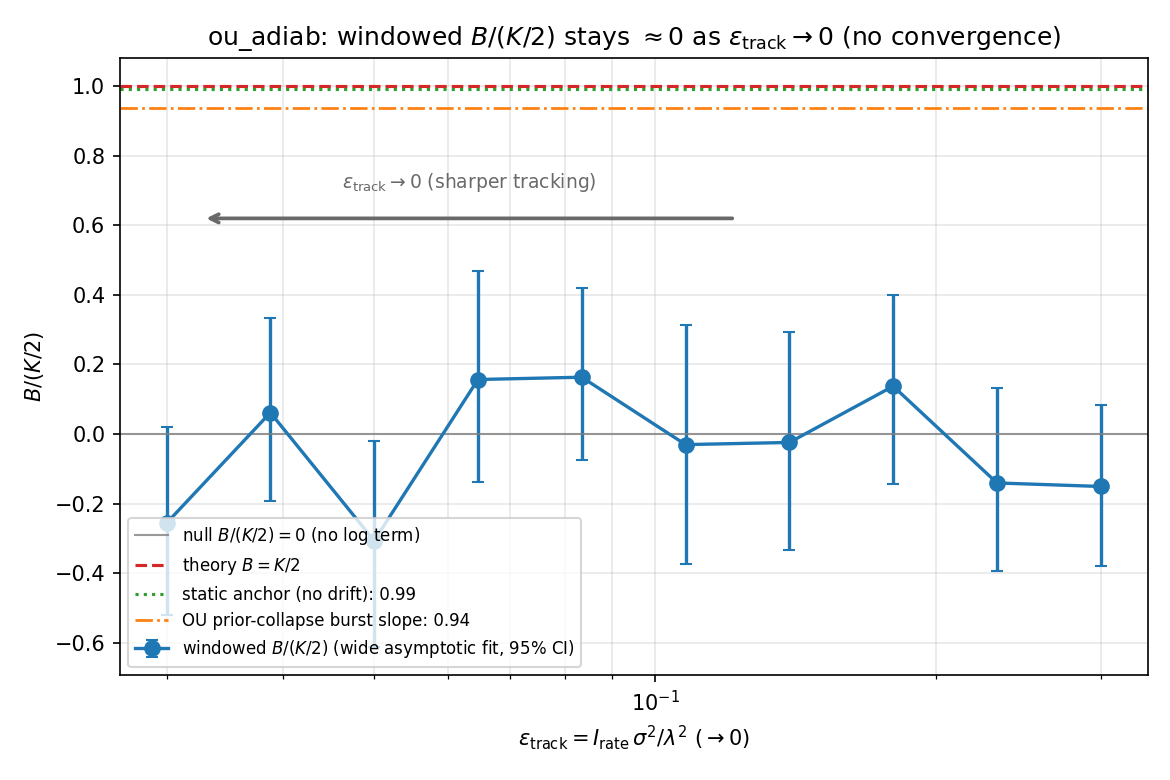
\includegraphics[width=0.82\linewidth]{figs/fig_ou_adiab_B_vs_eps.png}}

\caption{Структурная недостижимость наклона \(K/2\) (C1, Утверждение 1; серия \protect\texttt{ou\_adiab}). Отношение \(B/(K/2)\), оценённое в широком асимптотическом окне, остаётся плоским около нуля при понижении \(\epsilon_{\text{track}}\) на порядок --- а не растёт к \(1\) --- тогда как статический якорь (без дрейфа) даёт \(K/2\) (\(0{,}990\)), а транзиентный всплеск коллапса приора --- \(0{,}936\). Лог-несущее окно \(\sigma\)-инвариантно (\(W \approx 156\)--\(166 \approx\) const по всем 10 точкам; значения \(W\) приведены в § 6.1, на графике не отложены), поэтому предел \(\epsilon_{\text{track}}\to0\) его не открывает. Серая линия --- нулевая гипотеза \(B/(K/2)=0\) (лог-члена нет); все точки сидят на ней.}

\end{figure}



\emph{2. \texttt{fou\_floor} --- пол ностальгии и показатель скорости для дробного OU (Теорема 2).} Реальная траекторная симуляция на \textbf{точном стационарном fOU} (не пересчёт замкнутой формулы): \(K = 56\) независимых стационарных fOU-траекторий с \(H \in \{0{,}3,\ 0{,}5,\ 0{,}7,\ 0{,}9\}\) генерируются \textbf{спектрально-циркулянтным методом} из плотности \(S(\omega) \propto |\omega|^{1-2H}/(\lambda^2+\omega^2)\); собственные значения циркулянта Davies--Harte неотрицательны по построению (нулевое обрезание), целевая автоковариация \(\gamma(k)\) --- обратное ДПФ этих с.з. \textbf{Контроль ковариации} подтверждает \(\hat\rho(s) \approx \gamma(s)\) (отн. ошибка \(<5\%\) до лага \(\sim200\)--\(400\)). FIFO-память при \(\tau_E = 200\), \(c \approx 0{,}3\), \(|M| = 400\); бит предсказателен, пока \(\hat\rho^2(\text{возраст}) \ge \hat\rho^2(\tau_E)\).



\emph{Фактический результат прогона (seed 20260527, 40 реализаций, путь \(3{,}3\cdot10^4\), циркулянт \(M = 6{,}6\cdot10^4\)):} для всех \(H\) --- один и тот же пол \(\liminf\nu = 0{,}700 \approx 1-c\) (разброс по \(H\) ровно \(0{,}000\); рис. S2). Честная оговорка о \emph{статусе свидетельства} (асимметрия с \texttt{psp\_floor}): этот пол \emph{by-construction} --- детерминированный возрастной порог \(\hat\rho^2(\text{возраст}) \ge \hat\rho^2(\tau_E)\) пиннит долю свежих к \(c\), а значит пол к \(1-c\) тождественно; нулевой разброс --- следствие пиннинга, не независимое измерение (доказательство несёт § S2; § S4.5). Независимое содержание \texttt{fou\_floor} --- \emph{не} в значении пола, а в (i) контроле ковариации (пути --- подлинный стационарный fOU, не суррогат) и (ii) подтверждении \emph{показателя} \(4(1-H)\) в дальнем хвосте.



\textbf{Показатель скорости подтверждает аналитический \(4(1-H)\)} (рис. S4) --- на корректном процессе, в дальнем хвосте, по точной ковариации \(\gamma\) (выборочная ACF на долгой памяти смещена к нулю на больших лагах). В дальнем окне (\(\Delta \gtrsim 8\tau_E\)) локальный лог-лог-наклон \(\rho^2\) совпадает с \(4(1-H)\), и два \(H\) играют разную доказательную роль: \(H = 0{,}7\) (\(H < 3/4\), ∫β конечен) --- \emph{внутри} строгой Теоремы 2, совпадение \(1{,}237\) на \([8,40]\tau_E\) и \(1{,}201\) на \([20,80]\tau_E\) (аналитика \(1{,}2\)) --- \emph{внутритеоремное подтверждение}; \(H = 0{,}9\) (\(H \ge 3/4\), ∫β расходится) --- \emph{вне} теоремы, совпадение \(0{,}406\) и \(0{,}385\) (аналитика \(0{,}4\)) --- лишь \emph{численно поддержанная гипотеза}. В ближнем окне \([\tau_E, 8\tau_E]\) показатель не изолируется (\(1{,}62\) при \(H = 0{,}7\), \(0{,}46\) при \(H = 0{,}9\) по точной ковариации --- OU-«колено»; \(2{,}44\) и \(1{,}40\) по выборочной ACF --- смещение оценщика). \textbf{Это апгрейд C2:} прежний суррогат AR(1)\(\circ\)fGn давал \(2{,}23\) и \(1{,}26\) вне ДИ от \(4(1-H)\) --- свойство суррогата, не теории; на корректном fOU и глубина \((1-c)\), и показатель воспроизводятся. Качественная дихотомия держится: при \(H = 0{,}5\) хвост экспоненциальный (скорость \(4{,}07\cdot10^{-3}\)/шаг), при \(H > 0{,}5\) --- степенной. \emph{Фальсификатор:} расхождение пола \emph{по \(H\)} или дальне-хвостовой показатель вне \(4(1-H)\) (не наблюдается). Несущий вклад C2 --- \emph{глубина} \((1-c)\) --- воспроизведён инвариантно по \(H\); показатель вторичен и асимптотичен (§ 7 п. vi).



\emph{3. \texttt{psp\_floor} --- пол ностальгии для пуассоновского сброса (Теорема 2).} Реальная траекторная симуляция PSP-суррогата § 6.1 \cite{Andriishin2026b}: каждая координата несёт \emph{реализованный} пуассоновский поток сбросов интенсивности \(\mu = 1/\tau_E\); удержанный бит предсказателен, пока его координата фактически не сбросилась. Пол и скорость декорреляции читаются из реализованного процесса, а не из формулы \(e^{-\mu\Delta}\). \emph{Фактический результат прогона (seed 20260528, 40 реализаций, \(|M| = 400\), \(c \approx 0{,}3\), \(\mu \in \{10^{-3},\,3\cdot10^{-3},\,10^{-2}\}\)):} установившийся эмпирический пол \(\hat\nu_{\text{floor}} = 0{,}709\text{–}0{,}713 \approx 1-c\) на 10-кратном диапазоне \(\mu\) (разброс \(0{,}004\); рис. 2) --- инвариантность к частоте переключений подтверждена. Содержательная асимметрия с \texttt{fou\_floor}: здесь сброс --- \emph{реализованный} поток, а не зашитый порог, поэтому пол \(0{,}709\text{–}0{,}713\) --- \emph{независимое} свидетельство (систематически чуть выше теоретического \(0{,}70\)); \texttt{psp\_floor} несёт больше независимого содержания, чем by-construction \texttt{fou\_floor}. Скорость декорреляции по реализованной кривой выживания \(\hat S(\text{возраст})\) равна \(1{,}01\cdot10^{-3},\,3{,}01\cdot10^{-3},\,1{,}00\cdot10^{-2}\), каждый bootstrap-ДИ накрывает номинальный \(\mu\) --- настоящее измерение шкалы \(1/\mu\). Совместно \texttt{psp\_floor} (экспоненциальная \emph{скорость} \(\mu\)) и \texttt{fou\_floor} (степенной \emph{показатель} \(4(1-H)\)) упражняют оба конца класса перемешивания. \emph{Фальсификатор:} зависимость пола от \(\mu\) при фиксированном \(c\); скорость декорреляции вне ДИ от \(\mu\) (не наблюдается).



\begin{figure}

\centering

\pandocbounded{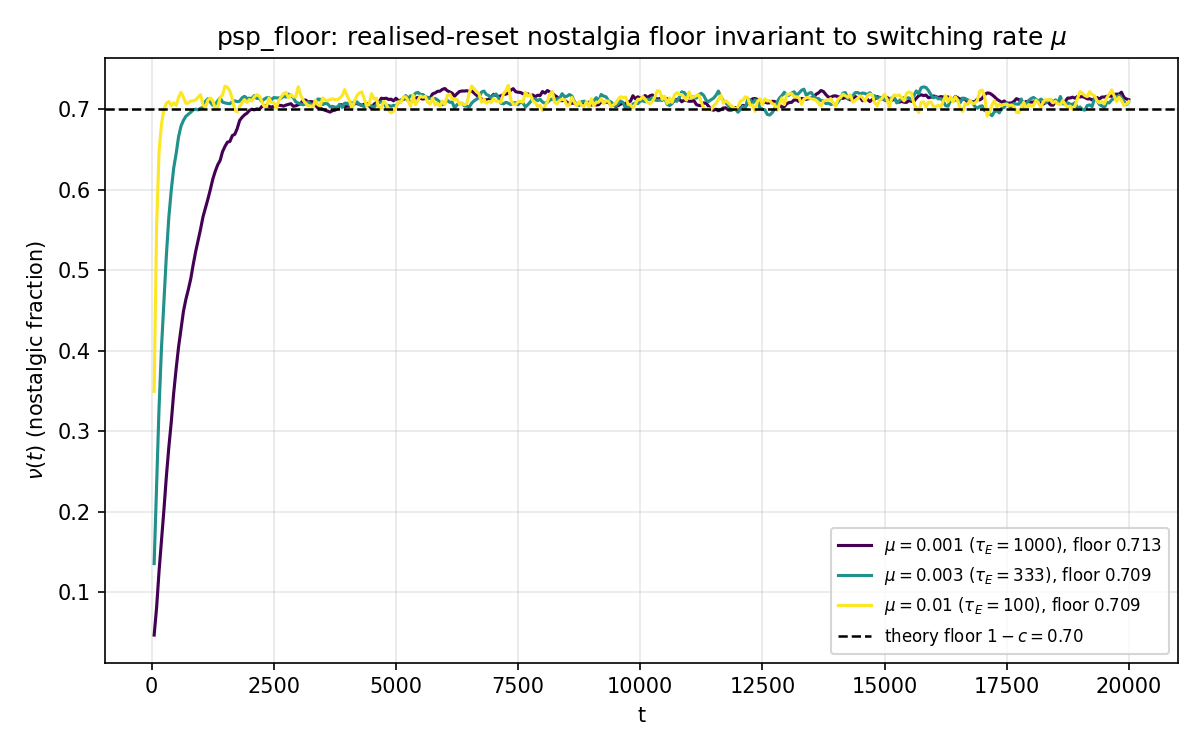
\includegraphics[width=0.82\linewidth]{figs/fig_psp_nu_vs_mu.png}}

\caption{Инвариантность глубины пола ностальгии по темпу обновления (C2, Теорема 2; серия \protect\texttt{psp\_floor} --- \emph{независимое} свидетельство). Установившийся пол \(\nu \approx 0{,}709\)--\(0{,}713 \approx 1-c\) один и тот же для интенсивности пуассоновских сбросов \(\mu\) на 10-кратном диапазоне (\(\tau_E = 1/\mu \in \{1000,333,100\}\)), при том что \emph{динамика выхода} на пол с \(\mu\) различна (видны три разные кривые). В отличие от by-construction-пола \protect\texttt{fou\_floor} (рис. S2), здесь сброс --- \emph{реализованный} пуассоновский поток, поэтому пол лежит чуть выше теоретического \(0{,}70\) --- независимое измерение глубины. Глубину задаёт темп обновления \(c\), не частота дрейфа.}

\end{figure}



\emph{4. \texttt{superlinear\_memory} --- фазовая граница (Теорема 3).} Память растёт как \(|M_{\le t}| \propto t^\alpha\) для \(\alpha \in \{1,\ 1{,}5,\ 2,\ 3\}\) и отдельно экспоненциально \(e^{\kappa t}\); измеряются \(\nu(t)\) и доля свежих \(\phi(t)\). \emph{Фактический результат прогона (seed 20260529, \(\tau_E = 200\)):} для всех полиномиальных \(\alpha\) доля свежих \(\phi(t) \sim t^{-\gamma}\) с \(\gamma \in \{1{,}000;\,0{,}991;\,0{,}982;\,0{,}964\}\) на baseline-окне, и префактор \(\phi\cdot t \to \alpha\tau_E\) (\(200,\,298,\,394,\,581\) против \(200,\,300,\,400,\,600\)), откуда \(\nu(t) \to 1\): полиномиального \(\alpha_c\) нет (рис. 3). Ведущий показатель тождественно \(\gamma = 1\); дрейф \(\gamma\) вниз с ростом \(\alpha\) --- конечно-оконная subleading-кривизна \(\phi = 1-((t-\tau_E)/t)^\alpha\), снимается расширением окна: \(\times10\) даёт \(\gamma \to \{1{,}000;\,0{,}999;\,0{,}998;\,0{,}996\}\), \(\times1000\) --- все \(1{,}000\) (диагностика \texttt{gamma\_window\_convergence}, § S4.4). Для экспоненциального роста (\(\kappa\tau_E \in \{0{,}1;\,0{,}5;\,1\}\)) --- \(\phi_\infty = 1-e^{-\kappa\tau_E} \in \{0{,}095;\,0{,}394;\,0{,}632\} > 0\) (ностальгия ниже \(1\)), но \(E_{\text{grow}}(t) \propto e^{\kappa t}\) расходится (отношение \(E_{\text{grow}}(T)/E_{\text{grow}}(0)\) до \(9{,}8\cdot10^{42}\)), и \(\eta_L(t) \to 0\) через знаменатель (5.3). \emph{Фальсификатор:} \(\phi(t)\), убывающая не как \(t^{-1}\) при полиномиальном росте, или насыщение \(\phi(t)\) при конечном \(\alpha\), опровергает отсутствие \(\alpha_c\).



\begin{figure}

\centering

\pandocbounded{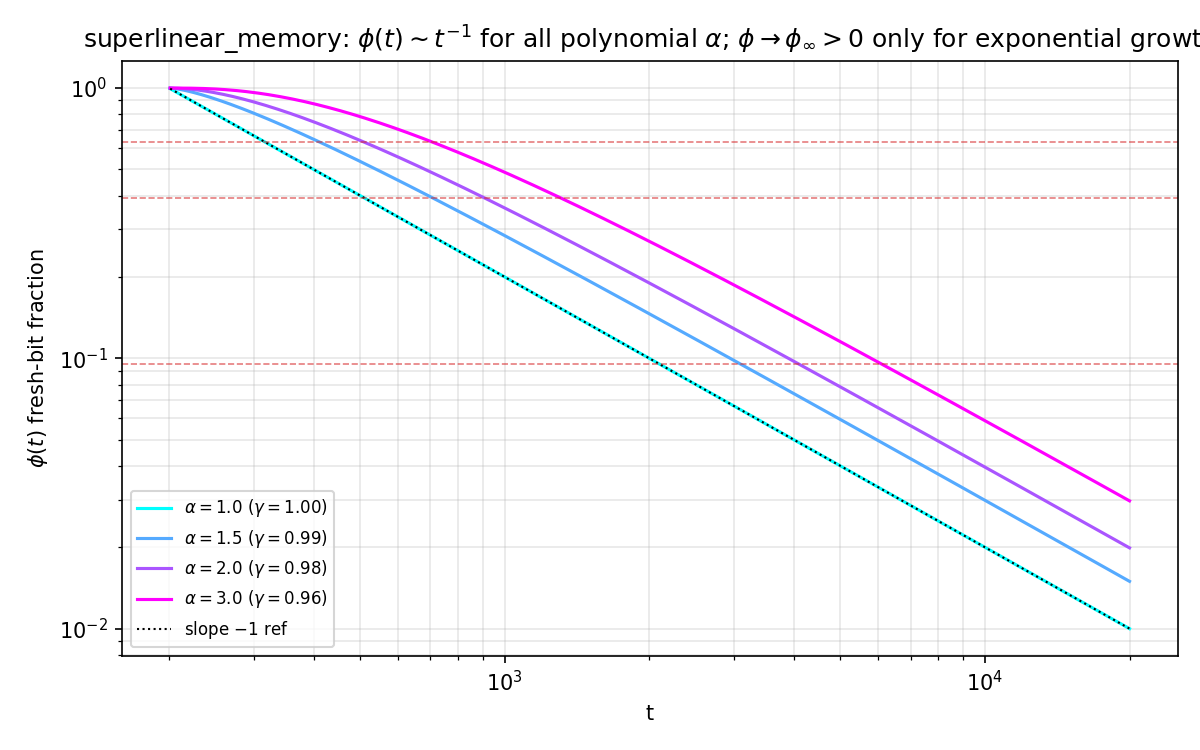
\includegraphics[width=0.82\linewidth]{figs/fig_superlinear_phi.png}}

\caption{Отсутствие конечного полиномиального порога \(\alpha_c\) (C3, Теорема 3; серия \protect\texttt{superlinear\_memory}). Доля свежих битов \(\phi(t) \sim t^{-\gamma}\) имеет ведущий показатель \(\gamma \equiv 1\) для всех полиномиальных \(\alpha \in \{1;1{,}5;2;3\}\) (префактор \(\phi\cdot t \to \alpha\tau_E\)), откуда \(\nu(t)\to1\) --- снос \emph{насыщается} при любом конечном \(\alpha\). Видимый дрейф \(\gamma\) вниз с ростом \(\alpha\) на исходном окне --- конечно-оконный subleading-артефакт точного \(\phi = 1-((t-\tau_E)/t)^\alpha\), снимающийся расширением окна фита (диагностика сходимости, § S4.4). Побег возможен лишь экспоненциальным ростом ёмкости --- рис. S6.}

\end{figure}



\emph{5. Чего симуляции не делают.} (i) Они \emph{не} доказывают теоремы --- это иллюстрации; строгие утверждения несут § S1--S3. (ii) Работают только с известным истинным \(\theta(t)\), поэтому \(\nu^{\text{theor}} = \nu^{\text{op}}\) по построению \cite{Andriishin2026b} § 6; операциональная неразличимость двух нормировок не тестируется. (iii) Не выходят за пределы абстрактных марковских цепей с дрейфом логитов. (iv) Сходимость \(B \to K/2\) проверяется на конечном скане --- поддержка, не доказательство. (v) Класс не-перемешивающихся (heavy-tailed) сред не симулируется --- вне области Теоремы 2.



\section{Обсуждение}\label{ux43eux431ux441ux443ux436ux434ux435ux43dux438ux435}



\emph{1. Связь с non-stationary online learning.} Кумулятивная избыточная потеря \(L_{\text{excess}}(t)\) --- это dynamic regret обучателя относительно оракула, отслеживающего дрейфующий оптимум, и Теорема 1 имеет прямую параллель в этой теории. Два бюджета изменения: (i) \emph{длина пути} \(P_T = \sum_t \|\theta(t)-\theta(t-1)\|\), введённая Зинкевичем \cite{Zinkevich2003}, который доказал dynamic-regret-границу \(O(\sqrt{T}\,(1+P_T))\) против дрейфующего сравнителя (и \(O(\sqrt T)\) против статического); Hall--Willett \cite{HallWillett2015} перенесли её на dynamic mirror descent в дрейфующих средах, а острую форму \(O(\sqrt{T(1+P_T)})\) с совпадающей нижней границей дали Zhang--Lu--Zhou \cite{ZhangLuZhou2018}; (ii) \emph{бюджет вариации} \(V_T\) в минимаксной теории Бесбеса--Гура--Зееви \cite{BesbesGurZeevi2015}, дающей \(\Theta(T^{2/3}V_T^{1/3})\). Для гладкого OU-дрейфа со стационарными приращениями оба бюджета растут линейно (\(P_T, V_T \propto T\)): минимаксная граница БГЗ даёт тогда ровно \emph{линейный} регрет \(\Theta(T)\), а tracking-граница Hall--Willett --- мажорирующую его суперлинейную верхнюю оценку \(O(T^{3/2})\). В обоих случаях это совместимо с линейным членом \(A\cdot t\) нашей декомпозиции (3.1): БГЗ воспроизводит его как ведущий, Hall--Willett мажорирует. Уточнение Теоремы 1 относится не к ведущему \(\Theta(T)\)-члену, а к \emph{суб-линейной} логарифмической поправке \((K/2)\ln(\lambda t)\) поверх него --- и именно она насыщается в плато (Утверждение 1). \emph{Логарифмический} регрет в этой линии достигается не у Зинкевича (\(\sqrt T\)), а для сильно-выпуклых потерь --- алгоритмами Хазана \cite{Hazan2007} и в дрейфующих средах \cite{HazanSeshadhri2009}; наша \((K/2)\ln\)-асимптотика ближе к этому классу. Различие форм (степенная БГЗ против логарифмической) отражает различие постановок: БГЗ ограничивают \emph{суммарную} вариацию, мы --- \emph{спектральную} структуру дрейфа. Структурно совпадает роль перемешивания (оптимальная шкала забывания \(\tau_f^{\text{forget}}\) настраивается под \(\tau_E\)) и монотонность по \(\tau_E\) \cite{Andriishin2026b} § S5.4. Связь dynamic-regret-границ \cite{CesaBianchiLugosi2006,Hazan2007} с \(\eta_L\) через тождество «regret = excess-loss = неоплаченная предсказательная ценность» заслуживает отдельного исследования.



\emph{1a. Необходимость сужения класса.} Теорема 2 расширяет область пола, но не отменяет фундаментального ограничения: без априорного ограничения класса дрейфа сублинейный динамический регрет недостижим --- при неограниченном бюджете вариации всякий обучатель несёт регрет не медленнее линейного \cite{BesbesGurZeevi2015,Zinkevich2003}. Условие перемешивания (4.1) --- необходимое сужение: оно отбирает среды, забывающие своё прошлое; вне его (heavy-tailed, не-возвратный дрейф) ни пол \(1-c\), ни адиабатическая асимптотика не гарантированы. Граница допустимого класса § 4 --- не недостаток, а отражение этой невозможности: снос неизбежен ровно для перемешивающихся сред, и это максимальный класс, на котором утверждение держится. В философском фоне это в духе no-free-lunch \cite{Wolpert1996}, но формально мы на NFL не опираемся (несущий аргумент --- невозможность sublinear dynamic regret); к тому же \cite{Wolpert1996} --- NFL \emph{супервизорного обучения}, усредняющий по классам целевых функций, а не по \emph{средам} с фиксированной спектральной структурой, поэтому применим лишь как аналогия.



\emph{1b. Размежевание с родственными понятиями.} Чтобы избежать ребрендинга, разведём три понятия. \emph{Ностальгия} --- удержание устаревшего слоя памяти, который более ничего не предсказывает, но \emph{продолжает оплачиваться} термодинамически. \emph{Catastrophic forgetting} \cite{McCloskeyCohen1989,Kirkpatrick2017} --- противоположная патология: \emph{потеря} всё ещё полезной памяти при дообучении. \emph{Concept drift} \cite{Gama2014} --- свойство самой \emph{среды} (смещение распределения), причина, а не следствие. Ностальгия не сводится к ним: она есть термодинамическая цена \emph{успешного} удержания (в отличие от forgetting) под действием дрейфа (concept drift как внешняя причина), и её предмет --- неоплачиваемость удержания, а не сохранность или утрата информации.



\emph{2. Калмановское слежение.} EWMA-фильтр Теоремы 1 --- частный случай стационарного фильтра Калмана--Бьюси для линейно-гауссовой системы со скрытым OU-состоянием \cite{KalmanBucy1961,AndersonMoore1979}; стационарная ошибка \(\Sigma_\infty \propto \sigma^2/\lambda\) (корень алгебраического Риккати) перенесена в термодинамический контекст как линейный коэффициент \(A\). Сам ненулевой \emph{steady-state tracking floor} --- классический \emph{lag misadjustment} адаптивной фильтрации \cite{Widrow1976,Haykin2014}. Наш вклад --- не существование флора, а его термодинамическое прочтение (флор \(\Leftrightarrow\) линейный член \(A\) и плато логарифма) и роль как информационной нижней границы \(n_{\text{eff}}\) (§ S1.6). Обобщение на нелинейную softmax-модель (расширенный/ансцентный Калман) --- техническое расширение, параллельное Замечанию 6 \cite{Andriishin2026b}.



\emph{3. Renewal theory.} PSP-класс Теоремы 2 --- процесс восстановления: точки сброса образуют пуассоновский поток, возрасты битов --- остаточные времена жизни. Равномерность распределения возрастов при FIFO (§ 4.2, § S2.0) --- следствие \emph{стационарного распределения возраста} буфера фиксированного размера (inspection paradox / backward recurrence time, \cite{Cox1962} гл. 5), а \emph{не} elementary renewal theorem. Степенное перемешивание fOU при \(H > 1/2\) соответствует heavy-tailed renewal --- естественное продолжение.



\emph{4. Что остаётся открытым.} (i) \emph{Heavy-tailed и не-марковский дрейф без перемешивания}: Теорема 2 требует \(\beta(s) \to 0\); среды с расходящейся автокорреляцией выпадают из класса, и пол \(1-c\) для них не гарантирован. (ii) \emph{Мост к fluctuation theorems}: декомпозиция бюджета на потоки \(E_{\text{store}}, E_{\text{grow}}, E_{\text{actual}}\) \cite{Andriishin2026b} (1) и теоремы Crooks/Jarzynski с feedback-контролем \cite{SagawaUeda2009}, неравенства для bipartite-систем и transfer entropy \cite{HartichBaratoSeifert2014}, стохастическая термодинамика вычисления \cite{Wolpert2019} (общий обзор информационной термодинамики --- \cite{Parrondo2015}) могут дать более тонкие неравенства для каждого потока --- направление для будущих работ. (iii) \emph{Операциональная versus теоретическая эффективность}: Теорема 1 доказана для контрфактической \(\eta_L^{\text{excess}}\); перенос на измеримую \(\eta_L(t)\) остаётся структурным. (iv) \emph{Строгий переходный фильтр}: вывод \(K/2\) опирается на стационарный Риккати и эвристику \(n_{\text{eff}} \asymp \lambda t\) (A3); строгий нестационарный Риккати и контроль остатка softmax-линеаризации (A1) за пределами адиабатического окна открыты. (v) \emph{Численная асимптотическая реализуемость \(B \to K/2\) (установлена как недостижимая)}: расширенная проверка с \emph{оптимальным} калмановским обучателем (§ 6.1, § S4.1) опровергла прежнюю внутреннюю рабочую гипотезу --- попытку толкнуть \(\epsilon_{\text{track}} \to 0\), чтобы восстановить \(\hat B \to K/2\) как наклон (опровергнута именно попытка, \emph{не} гипотеза § S8.1 \#2 \cite{Andriishin2026b}, которая лишь предполагала функциональную форму и Теоремой 1 аналитически подтверждена). При подлинном OU-дрейфе \(n_{\text{eff}}\) ограничен флором, \(L_{\text{excess}}\) выходит на плато, и в широком окне \(B/(K/2) \to 0\) (§ 6.1); препятствие структурно (\(\tau_{\text{conc}}\) и адиабатический потолок оба \(\propto 1/\sigma^2\)). Растущая память не спасает: флор есть MMSE-нижняя граница \(n_{\text{eff}}\) по всем архитектурам памяти (§ S1.6, § 3, Утверждение 1). Поэтому вопрос о растущей памяти не «открыт» и не «замкнут на C3», а \emph{снят} оптимальностью флора в окне A1 (наращивание сырья и бесплодно, и дорого --- режим Теоремы 3; не-гауссова модель открыта, п. iv). (vi) \emph{Эмпирический показатель скорости сноса fOU}: несущий вклад C2 --- \emph{глубина} пола \((1-c)\) --- доказан и от показателя скорости не зависит; \emph{показатель} \(4(1-H)\) вторичен и \emph{асимптотичен} --- на точном стационарном fOU подтверждается в дальнем хвосте (\(\Delta \gtrsim 8\tau_E\): \(1{,}20\) при \(H = 0{,}7\) против аналитики \(1{,}2\); \(0{,}39\)--\(0{,}41\) при \(H = 0{,}9\) против \(0{,}4\)), но в ближнем окне не изолируется (OU-«колено», смещённая выборочная ACF), и читается по точной ковариации (§ 6.2, § S4.2). Структурно это \emph{та же ситуация, что транзиентность в C1}; на корректном fOU (не суррогате AR(1)\(\circ\)fGn) и глубина \((1-c)\), и показатель воспроизводятся, что \textbf{усиливает} C2. Открыт лишь строгий контроль скорости сходимости при \(H \ge 3/4\) --- пол это не подрывает.



\section{Связь со статьями \#1 и \#2}\label{ux441ux432ux44fux437ux44c-ux441ux43e-ux441ux442ux430ux442ux44cux44fux43cux438-1-ux438-2}



Настоящая работа --- третий шаг программы ландауэровской эффективности самомоделирования и расширяет, а не пересматривает, оба предшественника.



\emph{Резюме без формул.} Снос неизбежен по одной простой причине: все три способа уйти от него упираются в одно и то же. Старое знание неизбежно перестаёт коррелировать с настоящим --- среда забывает своё прошлое, а вместе с ней обесценивается и записанная о нём память; платить же за хранение этой памяти приходится всё больше. Поэтому ни более точное слежение за средой, ни более быстрое обновление памяти, ни наращивание её ёмкости не спасают: три маршрута бегства перекрыты, и за ними стоят всего два механизма --- старая память декоррелирует, а цена её хранения растёт. Технический разбор этого замыкания --- ниже.



\emph{Неизбежность сноса как итог.} Три теоремы перекрывают три маршрута бегства, все три тупиковые (точное слежение --- no-go реализуемости Утверждения 1; обновление памяти --- универсальный пол \(1-c\) Теоремы 2; рост ёмкости --- отсутствие полиномиального порога Теоремы 3), и совокупно \(\eta_L \to 0\) неизбежно. Квалификатор уровня (из § 7 п. iv): no-go условен на постулатах самооплаты и стационарного учёта (A1)+(A3) \cite{Andriishin2026b} и линейно-гауссовом адиабатическом приближении; «неизбежность» доказана \emph{в адиабатическом окне} / \emph{для перемешивающихся сред} (\(\beta(\Delta t)\to0\), § 2.6, § 4) --- строгая версия за пределами класса (не-адиабатика, heavy-tailed дрейф) открыта (§ 4.6, § 7 п. i, iv). В этих границах устаревание нестационарной памяти --- не артефакт и не следствие субоптимальности, а структурное свойство: рациональный ответ --- не наращивать точность или ёмкость, а периодически \emph{сбрасывать} устаревший слой (оптимальный \(\tau_{\text{reset}}^*\) \cite{Andriishin2026b} (12), § 5 п. 6).



\emph{Взаимозамкнутость маршрутов.} Три маршрута перекрыты не \emph{независимо}, а \emph{взаимозамкнуто}: попытка уйти от одного либо бесплодна уже на информационном уровне, либо упирается в другой. Это снимает возражение, будто неизбежность условна --- «лишь для насыщающейся памяти», тогда как обучатель с \emph{растущей} памятью якобы поднял бы \(n_{\text{eff}}\) относительно \(\theta(t)\) выше флора \((1-g^\star)/g^\star\). Возражение неверно уже информационно: флор есть \emph{оптимум слежения} --- нижняя граница \(n_{\text{eff}}\) по всем архитектурам памяти, а не предел конкретной ёмкости (§ 7 п. v; § S1.6). Поэтому попытка поднять \(n_{\text{eff}}\) либо (i) информационно бесплодна (оптимальный фильтр уже на флоре --- C1, тот же декорреляционный механизм \(\beta(\Delta t)\to 0\), что несёт пол C2)\footnote{Флор говорит о декорреляции от \emph{текущего} \(\theta(t)\), а механизм Теоремы 2 (4.1) --- от \emph{будущей траектории} \(\theta_{[t,t+\tau]}\); для горизонта \(\tau = O(1)\) оба имеют один показатель затухания (для fOU траекторный супремум достигается на ближнем конце, сохраняя ведущий \(4(1-H)\)). Полный аргумент --- § S2.0, Замечание «траектория versus пара».}, либо (ii) субоптимальна наращиванием сырья --- бесплодно \emph{и} дорого (режим Теоремы 3: \(E_{\text{grow}}, E_{\text{store}} \propto e^{\kappa t}\), \(\eta_L \to 0\) через знаменатель (5.3)--(5.4)). Растущая память \emph{не открывает} четвёртого маршрута, и «неизбежность» \textbf{не условна} (в линейно-гауссовом окне A1; не-гауссова модель открыта, § 7 п. iv). Маршруты --- три грани одного замкнутого контура; несущих механизмов \emph{два} (mixing-пол и бюджетный канал, развёрнуто ниже), C1 замкнут на mixing через флор слежения.



\emph{Что строго ново как целое.} Каждый отдельный кирпич честно атрибутирован (§ 3 п. 6 --- флор как класс II BNT; § 4 п. 3 --- DPI-механизм пола; § 5 п. 5a --- насыщающая часть ⊂ C2), поэтому самостоятельный вклад работы --- \emph{не} в любом одном результате, а в \emph{замыкании контура}. Три a-priori-независимых маршрута сводятся к \emph{двум} несущим механизмам, оба перекрытые поверх ландауэровского знаменателя: (i) \emph{mixing-пол} --- декорреляция, ставящая и пол ностальгии (C2), и флор слежения (C1), и несущая через поточечное S2.0 насыщающую часть C3 (§ 5 п. 5a); (ii) \emph{бюджетный канал} --- расходящаяся цена роста ёмкости \(E_{\text{grow}} + E_{\text{store}} \propto e^{\kappa t}\) (несущая новизна C3, § 5 п. 4), которой нет у C2. Это не три позитивных результата, а \emph{теорема о замкнутости} маршрутов бегства (no-go синтеза), и само замыкание есть проверяемое предсказание --- обнуление \(\hat B\to0\) в широком окне (§ 6), которое подтверждается. Сверх статьи \#2 строго новы три вещи: (i) DPI-обобщение пола со спектральной щели OU на общее перемешивание (захват не-марковского fOU через множественную, а не парную, корреляцию --- § 4); (ii) бюджетный канал расходимости цены роста ёмкости, отсутствующий у \#2 (§ 5 п. 4); (iii) демонстрация, что три маршрута \emph{не} независимы, --- и это, а не любой из них поодиночке, есть структурный результат работы.



Не образует четвёртого маршрута и квазистационарный предел очень медленного дрейфа \(\lambda \to 0\), в котором \(n_{\text{eff}} \sim t\) мог бы расти (\(\tau_E = 1/\lambda \to \infty\) уносит горизонт устаревания в бесконечность). При сохранении адиабатичности этот предел \emph{непрерывно вырождается в стационарный режим}, где сноса нет \emph{по определению}, а не преодолён: рост \(n_{\text{eff}} \sim t\) есть исчезновение самого дрейфа, и флор \(1/g^\star \to \infty\) вместе с \(g^\star \propto \sigma^2 \to 0\) перестаёт быть ограничением. Ни конечный \(\lambda\) (флор активен), ни предел \(\lambda \to 0\) (дрейф исчезает) побега не открывают.



\emph{Отношение к статье \#2 \cite{Andriishin2026b}.} Все три теоремы продвигают открытые вопросы § 8.5 \cite{Andriishin2026b}, не вступая с ней в противоречие. Теорема 1 \emph{разрешает} аспект (i) гипотезы § S8.1 \emph{отрицательно}: значение \(B = K/2\) подтверждается в пределе \(\epsilon_{\text{track}}\to 0\) \emph{как транзиентное} (реализуемое лишь на окне \(t\lesssim\tau_{\text{conc}}\)), но достижимой асимптотической реализации наклона при дрейфе не существует (no-go, Утверждение 1) --- разрешение открытого вопроса, а не опровержение; перенос на операциональную \(\eta_L\) открыт (§ 6.1, § 7). Теорема 2 \emph{вкладывает} Лемму 2 как частный случай \(H = 1/2\): спектральная щель OU --- достаточное, но не необходимое условие пола; необходимое --- перемешивание (4.1). Теорема 3 закрывает вопрос о сверхлинейной памяти: побег невозможен полиномиально и термодинамически дорог экспоненциально. Аппарат \cite{Andriishin2026b} (\(\eta_L\), \(N_{\text{max}}\), \(\nu\), OU-параметризация, decomposition) используется без переопределения.



\emph{Отношение к статье \#1 \cite{Andriishin2026a}.} Стационарная лемма \cite{Andriishin2026a} § 2.1 --- частный случай нестационарного бюджета при \(\dot E_{\text{store}} = \dot E_{\text{grow}} = 0\) \cite{Andriishin2026b} § 2.2. В стационарном пределе нулевого дрейфа \emph{дрейф-индуцированная} ностальгия \(\nu \to 0\) и \(L_{\text{excess}}\) не растёт логарифмически --- обе теоремы вырождаются в стационарную картину. Во избежание смешения механизмов: это \(\nu \to 0\) \emph{не} отменяет «nostalgia-биты» леммы \#1, возникающие из иного механизма --- стока конечной памяти (удержание сверх корреляционного масштаба даже без дрейфа), ненулевого и в стационарном пределе. Механизмы ортогональны: дрейф-индуцированный снос исчезает при нулевом дрейфе, сток конечной памяти --- нет.



\emph{Прогрессивность расширения.} Программа удовлетворяет лакатошскому критерию прогрессивности: каждая работа добавляет избыточное, независимо проверяемое содержание. Статья \#1 --- стационарная шкала; статья \#2 --- нестационарное расширение с тремя открытыми вопросами; настоящая работа --- три теоремы, сводящие три маршрута бегства в единый тезис неизбежности. Отрицательный результат (Утверждение 1) --- \emph{прогрессивный}, а не дегенеративный сдвиг: он не спасает гипотезу § S8.1 вспомогательной правкой, а делает проверяемое предсказание (\(\hat B \to 0\) в широком окне, § 6), которое подтверждается. Работа порождает новые открытые задачи (скорость сходимости к \(4(1-H)\) при \(H \ge 3/4\); heavy-tailed дрейф; мост к fluctuation theorems) для будущих работ. Операционализация с \emph{растущей} памятью открытой задачей здесь \emph{не} остаётся --- она закрыта оптимальностью флора, не образуя независимого маршрута (§ 7 п. v).



\emph{Субстрат-независимость.} Снос --- свойство информационной термодинамики нестационарной памяти, а не конкретного носителя: ни потолок числителя (\(I_{\text{pred}} \le \ln k\)), ни расходимость знаменателя (ландауэровский бюджет) не зависят от того, хранится ли память синапсами, весами сети или эпигенетической меткой. Отсюда единое прочтение того, почему адаптивные системы на разных субстратах сходятся к одной стратегии --- периодически \emph{сбрасывать} устаревший слой, а не накапливать память без предела (continual-обучение с replay, синаптический оборот, эволюционное bet-hedging --- § 5 п. 6, § 7 п. 1b): кандидаты на проявление одного и того же no-go. Это параллель, а не вывод --- теоремы доказаны лишь в своём модельном классе (перемешивающийся медленный дрейф, адиабатическое окно A1), а проверка на конкретных системах остаётся отдельной задачей.



\section*{Декларации}
\textbf{Funding.} No external funding was received for this research.



\textbf{Competing interests.} The author declares no competing interests.



\textbf{Author Contributions.} Sole author (A.A.): conceptualization, proofs, numerical design, and writing.



\textbf{Data Availability.} Код численных симуляций (§ 6) и исходные файлы работы открыто доступны в публичном репозитории-зеркале \texttt{andriishin/landauer-undertow-oa} (GitHub) и архивированы на Zenodo (DOI 10.5281/zenodo.20836705). Внешних эмпирических данных работа не использует (теоретическая работа с численными иллюстрациями на абстрактных моделях).



\textbf{AI disclosure.} The author used an AI assistant (large language model) as a tool for drafting, literature cross-referencing, and editing under the author's direct supervision. All mathematical results, proofs, and scientific claims were conceived, verified, and approved by the author, who takes full responsibility for the content.




\section*{References}
\bibliographystyle{iopart-num}
\bibliography{refs}

\end{document}
